% --- Template for thesis / report with tktltiki2 class ---
% 
% last updated 2013/02/15 for tkltiki2 v1.02

\documentclass[finnish]{tktltiki2}

% tktltiki2 automatically loads babel, so you can simply
% give the language parameter (e.g. finnish, swedish, english, british) as
% a parameter for the class: \documentclass[finnish]{tktltiki2}.
% The information on title and abstract is generated automatically depending on
% the language, see below if you need to change any of these manually.
% 
% Class options:
% - grading                 -- Print labels for grading information on the front page.
% - disablelastpagecounter  -- Disables the automatic generation of page number information
%                              in the abstract. See also \numberofpagesinformation{} command below.
%
% The class also respects the following options of article class:
%   10pt, 11pt, 12pt, final, draft, oneside, twoside,
%   openright, openany, onecolumn, twocolumn, leqno, fleqn
%
% The default font size is 11pt. The paper size used is A4, other sizes are not supported.
%
% rubber: module pdftex

% --- General packages ---

\usepackage[utf8]{inputenc}
\usepackage[T1]{fontenc}
\usepackage{lmodern}
\usepackage{microtype}
\usepackage{amsfonts,amsmath,amssymb,amsthm,booktabs,color,enumitem,graphicx}
\usepackage[pdftex,hidelinks]{hyperref}
\graphicspath{ {images/} }
% Automatically set the PDF metadata fields
\makeatletter
\AtBeginDocument{\hypersetup{pdftitle = {\@title}, pdfauthor = {\@author}}}
\makeatother

% --- Language-related settings ---
%
% these should be modified according to your language

% babelbib for non-english bibliography using bibtex
\usepackage[fixlanguage]{babelbib}
\selectbiblanguage{finnish}

% add bibliography to the table of contents
\usepackage[nottoc]{tocbibind}
% tocbibind renames the bibliography, use the following to change it back
\settocbibname{Lähteet}

% --- Theorem environment definitions ---

\newtheorem{lau}{Lause}
\newtheorem{lem}[lau]{Lemma}
\newtheorem{kor}[lau]{Korollaari}

\theoremstyle{definition}
\newtheorem{maar}[lau]{Määritelmä}
\newtheorem{ong}{Ongelma}
\newtheorem{alg}[lau]{Algoritmi}
\newtheorem{esim}[lau]{Esimerkki}

\theoremstyle{remark}
\newtheorem*{huom}{Huomautus}


% --- tktltiki2 options ---
%
% The following commands define the information used to generate title and
% abstract pages. The following entries should be always specified:

\title{Reunalaskenta arkkitehtuurit}
\author{Lauri Vene}
\date{\today}
\level{Pro gradu -tutkielma}
\abstract{Tiivistelmä.}

% The following can be used to specify keywords and classification of the paper:

\keywords{reuna, pilvi, tietojenkäsittelytiede}

% classification according to ACM Computing Classification System (http://www.acm.org/about/class/)
% This is probably mostly relevant for computer scientists
% uncomment the following; contents of \classification will be printed under the abstract with a title
% "ACM Computing Classification System (CCS):"
% \classification{}

% If the automatic page number counting is not working as desired in your case,
% uncomment the following to manually set the number of pages displayed in the abstract page:
%
% \numberofpagesinformation{16 sivua + 10 sivua liitteissä}
%
% If you are not a computer scientist, you will want to uncomment the following by hand and specify
% your department, faculty and subject by hand:
%
% \faculty{Matemaattis-luonnontieteellinen}
% \department{Tietojenkäsittelytieteen laitos}
% \subject{Tietojenkäsittelytiede}
%
% If you are not from the University of Helsinki, then you will most likely want to set these also:
%
% \university{Helsingin Yliopisto}
% \universitylong{HELSINGIN YLIOPISTO --- HELSINGFORS UNIVERSITET --- UNIVERSITY OF HELSINKI} % displayed on the top of the abstract page
% \city{Helsinki}
%


\begin{document}

% --- Front matter ---

\frontmatter      % roman page numbering for front matter

\maketitle        % title page
\makeabstract     % abstract page

\tableofcontents  % table of contents
\

% --- Main matter ---

\mainmatter       % clear page, start arabic page numbering

\section*{Huomioita}
\begin{itemize}
\item reuna
\item reunasolmu
\end{itemize}

Tutkielmassa puhutaan mobiililaitteesta, mutta monet toiminnallisuudet ovat sovellettavissa kaikenlaisiin mobiileihin laitteisiin, esimerkiksi kannettaviin tai älykkäisiin ajoneuvoihin. 

Listan Mobile Computingin neljästä pääasiallisesta rajoitteesta.\\
\textit{Unpredictable variation in network quality, lowered trust and robustness of
mobile elements, limitations on local resources imposed by
weight and size constraints, and concern for battery power
consumption} [13]

[13]M. Satyanarayanan, "Fundamental Challenges in Mobile Computing," Proc.
15th ACM Symp. Principles of Dist. Comp., Philadelphia, PA, May, 1996



\section{Johdanto}

\section{Reunalaskennan perusteet}

\subsection{Motivaatio}
Reunalaskennan ideana on täydentää ja avustaa resurssiköyhiä asiakaslaitteita. Mobiililaitteisiin voitaisiin teoriassa lisätä enemmän resursseja, mutta ne tulisivat kannettavuuden ja käyttöajan kustannuksella. 
Avustamiseksi voidaan ajatella esimerkiksi tilanne, jossa akkuvirtaa säästääkseen, mobiililaite välittää resurssi intensiivisen laskutoimituksen reunasolmulle laskettavaksi. Reunasolmun voi ajatella kevennetyksi versioksi palvelimesta joten sen rajoitteet ovat hyvin erilaiset kuin asiakaslaitteen.
Täydentävä toiminta reunalaskennan avulla tarkoittaa asiakaslaitteen resurssin puutetta suoriutua jostakin tehtävästä. Esimerkiksi muistin riittämättömyys kuvankäsittelyyn. Tällöin voitaisiin esimerkiksi ottaa etäkäyttöyhteys reunasolmuun jolla käsittely tehdään. Asiakaslaitteelle jäisi tässä tilanteessa tehtäväksi ainoastaan esittää reunasolmun tilaa käyttäjälle.


Satyanarayana \cite{RefWorks:doc:5a65a2cee4b0cb152cfb50e7} esitti artikkelissaan pervasive computing esimerkkejä jokapaikan tietotekniikasta. Ympäristöön sijoitettujen laitteiden yhteistoiminnan avulla, asiakkaalle voidaan tarjota parempaa ja täsmällisempää palvelua. Yhtenä palvelun laadun ehtona on kyky ennakoida asiakkaan toimintaa.
Nykyään mobiililaitteilla on mahdollista hyödyntää langattomia yhteyksiä.
Suurin osa palvelinresursseista ja palveluiden tuottamiseen käytettävästä tiedosta  on keskittyneenä pilveen. Käytännössä minkä tahansa palvelun käyttäminen mobiililaitteella edellyttää yhteyttä näihin pilvipalveluihin. Pilvipalveluiden ylläpitäminen  

 Satyanara etal. argumentoivat julkaisussaan että verkon lantenssia ei voida enää juurikaan pienentää. Ratkaisuksi jää palveluiden tuominen lähemmäksi.

Toinen painopiste on siinä että tieto seuraa käyttäjää. Esimerkiksi pöytäkoneelta mobiililaitteeseen.(Satyanarayanan, 2001).
Cyber foraging, on termi jota käytetään kuvaamaan paradigmaa jossa laite etsii ympäristöstä hyödynnettävää tietoa ja avustajia/korvikkeita. Avustajan (surrogate) rooli on täydentää lähtökohtaisesti resurssirajallista laitetta, esimerkiksi suorittamalla laskentaa, jotta asiakaslaite voisi esimerkiksi säästää akkua.
Tähän toimintaan liittyy kuitenkin useita haasteita. Esimerkiksi kuinka asiakaslaite löytää avustajan? Mitäs jos avustaja on ruuhkautunut? Kuinka avustaja alustetaan ja kauanko siinä kestää? 
Nämä ovat keskeisiä kysymyksiä myös reunalaskennassa. 
Vastuun jakaminen asiakaslaitteen sekä reunanklusterin välillä on riippuvainen siitä, kuinka paljon avustusta asiakaslaite tarvitsee. 
Toiseen ääripäähän vietynä asiakaslaite on niin sanottu kevyt asiakaspääte (thin client), jolla ei olisi resursseja juurikaan mihinkään. Tällainen asiakaslaite joutuisi jakamaan kaiken laskennan eteenpäin avustajalle. 
Tämän kaltainen asiakaslaite olisi riippuvainen reunan mahdollisuuksista suorittaa palveluiden vaatimia toiminnallisuuksia. 
Seuraavana askeleena kohti itsenäisempää suoriutumista olisi asiakaslaite, joka pystyy osittain tarjoamaan käyttäjälle palveuita. Tämä laite tarvisi reunaklusterilta avustusta ainoastaan joissain tapauksissa. 
Viimeisenä toimijana olisi kokonaan itsenäinen asiakaslaite, joka tarvitsisi reunalta ainoastaan palveluita täydentäviä ominaisuuksia.
Tämä laite saattaisia turvautua reunalaskentaan esimerkiksi jos akku on vähissä, tai laitteella itsellään ei ole kaikea tarvittavaa tietoa laskennan suorittamiseksi.

\subsection*{a}
\begin{itemize}
\item Mistä reunalaskenta koostuu? (Suurimmat toimijat, keskeisimmät toiminnot)
\item Mikä on MEC?
\item Reunalaskenta vai reunapalvelu?
\item MCC vai MEC?
\item Pilvi vai palvelinkeskus, palvelinresursseja.
\item Mitä reunalaskenta on?
\item Miksei siirretä laskentaa pilveen?
\item Mitkä ovat mobiilin ongelmat nykyisellään?
\item Mitkä ovat reunalaskennan haasteet?
\end{itemize}


Pilvipalvelulla tarkoitetaan palvelua, joka sijaitsee internetissä. Palvelut tarjotaan käyttäjälle verkkoyhteyden välityksellä.
Pilvipalvelut sisältävät usein suuria määriä laskenta- ja tallennusresursseja. Palvelut usein sijoitettu siten että ne ovat runkoverkossa kiinni, jolloin niiden voidaan ajatella sijaitsevan internetin "keskustassa".
Yleensä palveluita ylläpidetään keskitettyinä korkeintaan muutamaan eri konesaliin.
Pilvipalvelun palvelun kohde on usein asiakaslaite (UE, user equipment), joka sijaitsee internet-topologian näkökulmasta lehtisolmussa.

Reunalaskenta on yksi hajautetun laskennan muoto jossa 

Mobiililaitteiden yleisiä ominaisuuksia ovat resurssien vähyys ja akkuvirran rajallisuus. Mobiililaitteiden käyttö on myös usein riippuvaista langattomista verkkoyhteyksistä.
Palveluiden toiminta mobiililaitteilla on siis riippuvainen näiden kolmen ominaisuuden asettamista rajoista.
Laskentaresurssien lisääminen johtaisin lyhyempään käyttöaikaan akkuvirralla. Suurempi akku mahdollistaa pidemmän käyttöajan, mutta se tekisi laitteesta suuremman. Akun kokoa ja laskentaresurssien määrää pyritäänkin tasapainottamaan.
Voidaan pyrkiä minimoimaan laitteen virrankulutus esimerkiksi laittamalla laitteeseen heikkotehoisempi suoritin. Tämä näkyy siinä, millaisia palveluita mobiililaitteella voidaan tarjota.
Esimerkiksi kuvankäsittelyä tai muuta raskaampaa laskentaa vaativaa toiminnallisuutta ei voida tällaisella laitteella tehdä. 
Seuraava vaihtoehto olisi lähettää laskentaa tehokkaammille laitteille pilveen. Laskennan siirtäminen vie aikaa ja tällöin ei voida tarjota kovin reaaliaikaisia palveluita.
Siirrettyyn laskentaan kuluva aika koostuu pääasiassa verkon viiveestä, siirrosta ja itse laskennasta. 
Kokonaisuudessa siirtämiseen ja laskentaan kuluvan ajan määrään vaikuttaa pilven sijainti, verkon ruuhkaisuus, verkon kapasiteetti, sekä käytössä olevan laskentakapasiteetin määrä.
Reunalaskenta on konsepti, jonka avulla laskenta voidaan tuoda lähemmäksi käyttäjää.

Reunalaskennassa (MEC,Mobile Edge Computing vai MCC Mobile Cloud Computing?) on tarkoitus tuoda palvelinresursseja lähemmäksi käyttäjää. Reunalaskenta on osassa kirjallisuutta jaettu kahteen kategoriaan sen mukaan tarjotaanko palvelua RAN (Radio access network) vai yleisesti WAN yhteydessä. RAN verkossa toimivaa reunalaskentaa kutsutaan Multi-access edge computing ja muita reunalaskennan ratkaisumalleja  nimillä kuten sumu(fog computing) tai cloudlet\cite{taleb2017multi} .
Tässä kontekstissa reunalla tarkoitetaan käyttäjän ja pilven väliin jäävää tilaa. TCP/IP-mallissa sovellustasolla olevia toimintoja ei siis esiinny tällä välillä.
Reunalaskenta siis mahdollistaa palveluiden tuottamisen lähempänä käyttäjää. Lähempänä on hieman harhaan johtava termi, koska mikä tahansa pilveä lähempänä oleva palvelu on lähempänä, eikä siis välttämättä konkreettisesti lähellä. 

Reunalaskennalle ei vielä ole olemassa kokonaisvaltaista arkkitehtuuria.
Ongelmakentän voi jakaa karkeasti kahteen osaan. Fyysiseen arkkitehtuuriin ja sovellustason arkkitehtuuriin. Nämä ovat toisistaan riippuvaisia.
Arkkitehtuuriratkaisut ovat riippuvaisia tarjottavista palveluista. Toiset arkkitehtuuriratkaisut tukevat toisia palveluita paremmin kuin toiset, kompromisseilta on siis vaikea välttyä.


\subsection{Keskeiset käsitteet}
Tässä kappalessa esitellään (mobiilin) reuna-arkkitehtuurin keskeiset käsitteet ja toimijat. 
Koska reunajärjestelmä sijoittuu osaksi olemassa olevaa hierarkiaa, esitellään myös reunan läheisyydessä sijaitsevat toimijat.
Reunan itsensä lisäksi käsitellään siis asiakaslaitteet ja pilvi, niiltä osin kuin ne liittyvät reunajärjestelmän käyttöön tai toimintaan.
Lähes kaikki tässä tutkielmassa esiteltävät reuna-arkkitehtuurit sijoittuvat mobiiliverkkoon. Tästä syystä esitellään LTE-mobiiliverkon toimijat ja siihen kuuluvat käsittet. 
Lopuksi määritellään mitä tässä tutkielmassa tarkoitetaan reuna-arkkitehtuurilla.

%Perinteinen asiakas-palvelin -malli koostuu vain kahdesta toimijasta. Reunajärjestelmän lisääminen tähän malliin luo omanalaisen hierarkian joka, muistuttaa enemmänkin asiakas-reuna-palvelin muotoista järjestelmää.
%Seuraavaksi käydään läpi hieman tarkemmin mitä nämä osat sisältävät ja mikä niiden keskeisin rooli reunajärjestelmän kontekstissa on. 
 


%Tähän voisi laittaa kuvan komponenttien asemmoitumisesta toisiinsa.
\subsubsection{Asiakaslaite}
Asiakaslaite (user equipment) on yleisnimitys laitteelle, joka on reunan tai pilven tarjoamien palveluiden asiakas. 
Asiakaslaitteen tyyppiä ei ole rajattu ja asiakaslaite voi olla esimerkiksi älypuhelin, älylasit tai vaikka verkkoyhteydellä varustettu auto. 
Yhdistävänä tekijänä on siis jonkinlainen yhteys reuna- tai pilvipalveluihin. Yleisesti yhteys on tyypiltään langaton. 
Tässä tutkielmassa asiakaslaitteella tarkoitetaan älypuhelinta, jollei toisin mainita.

Verkkohierarkian näkökulmasta asiakaslaitteet ovat lehtisolmuja. Tämä tarkoittaa että asiakaslaitteet toimivat ainoastaan palveluiden kuluttajina eivätkä siis tarjoa itse palveluita. Myöskään kulutettavien palveluiden tyypillä ei ole juurikaan merkitystä, kun asiaa käsitellään infrastruktuuri/arkkitehtuuritasolla.

Esimerkkinä asiakaslaitteen toiminnasta reunapalvelua hyödyntäen voisi olla ajoneuvo, joka käyttää reunapalveluita tiedon välittämiseen muille lähistöllä oleville ajoneuvoille.


%Asiakaslaite on yleisnimitys laitteelle, joka hyödyntää reunan tai pilven tarjoamia palveluita jonkin tietoliikenneyhteyden avulla.
%Reunalaskentaa käsittelevässä kirjallisuudessa asikaslaitteeseen viitataan usein UE (User Equipment) termillä. 
%Se mitä konkreettista laitetta asiakaslaitteella tarkoitetaan riippuu kontekstista. 
%Tässä tutkielmassa asiakaslaitteella tarkoitetaan älypuhelinta jollei toisin mainita. 
%Esimerkkinä jostain toisesta asiakaslaitteesta on auto, joka on varustettu mobiiliverkkoyhteydellä. Auto voi käyttää reunapalveluita esimerkiksi kommunikoidakseen muiden lähistöllä olevien autojen kanssa.
%Asiakaslaitteet verkkoyhteyksien muodostaman hierarkian "lehtisolmuja" joka tarkoittaa että ne eivät enää tarjoa palveluitaan muille asiakaslaitteille. 


\subsubsection{Reuna} \label{reunatoimijat}
Reuna koostuu useista toiminnallisista entiteeteistä, jotka voidaan jakaa sekä fyysisiin, että loogiisin entiteetteihin. On kuitenkin hyvä ymmärtää koko reunan käsittävä reuna-alue, joka esitellään ensimmäisenä. Tämän jälkeen esitellään reunasolmu, joka on reunajärjestelmän keskeisin fyysinen rakennuspalanen. Lopuksi esitellään pääasiassa ohjelmallisen tason toimivat toimijat reuna-alusta ja reunasovellus.

\paragraph{Reuna-alue} 
Reuna-alue tai reuna ei ole mikään tarkasti rajattu alue, vaan reunalla usein tarkoitetaan jonkin tietyn kontekstin mukaista reunaa. 
Yleisesti reunalla voidaan viitataan alueeseen, joka ulottuu asiakaslaitteelta runkoverkkoon asti. Reunalle ei siis ole tarkkaa määritelmää.
Reuna-alue rajautuu siinä esiintyvien toimijoiden mukaan jollekkin välille. 
Esimerkiksi mobiiliverkon tukiasemien yhteyteen rakennettua reunajärjestelmää käsiteltäessä, reunalla tarkoitetaan ainoastaan reunajärjestelmän asiakaslaitteita palvelevien osien muodostamaa vyöhykettä. 
Yleisenä nyrkkisääntönä voidaan pitää verkkoyhteyksien viivettä, suhteessa muuhun internettiin, koska reuna-alueella viiveiden tulisi siis olla muuta internettiä nopeampia. Toisin sanoen palveluiden tulisi sijaita lähempänä.


\paragraph{Reunasolmu} 
Tämän tutkielman kontekstissa reunasolmulla (mobile edge host) tarkoitetaan yksittäistä reunalaskentaa suorittavaa entiteettiä. Reunasolmu voi koostua esimerkiksi mobiilitukiaseman ja palvelinlaitteiston muodostamasta kokonaisuudesta. Reunasolmu sisältää vähintään reunasovelluksien suorittamiseen tarvittavan laitteiston, sekä toiminnallisesti reunasovelluksien suorittamiseen tarvittavat hallinnolliset toimet. 
Kuten aiemmin mainittu, reunajärjestelmä koostuu joukosta reunasolmuja, jotka on hajautettu maantieteellisesti.
Reunasolmut siis eroavat toisistaan vähintään sijainnin perusteella, mutta voivat erota myös käytettävissä olevien laskenta ja tallennus resurssien osalta.
Reunasolmun sijaintiin vaikuttaa käytössä oleva reuna-arkkitehtuuri.
%Kuten juuri mainittu, reunasolmujen sijaintiin vaikuttaa käytettävä reuna-arkkitehtuuri. 
Teoriassa reunasolmu voi sijainta asiakaslaitteesta \textit{yhden hypyn päässä}, jolloin asiakaslaitteella olisi suora yhteys reunasolmuun, mutta on myös mahdollista, että reunasolmu sijaitsee kauempana esimerkiksi runkoverkon reunalla. 
Laskentaresurssien osalta reunasolmu voi olla mitä tahansa vähäisillä laskenta ja tallennus resursseilla varustetun WiFi-tukiaseman ja kokonaisen palvelinklusterin väliltä. 

\paragraph{Reuna-alusta}
(Edge platform) on ohjelmistotason toimija, joka tarjoaa rajapinnan reunasovelluksien suorittamista varten. Toisin sanoen siis tarjoaa reunasovelluksille toimintaympäristön.
Reuna-alustan tehtävät eivät rajaudu ainoastaan yksittäiseen reunasolmuun, vaan sen lisäksi se hoitaa hallinnollisia tehtäviä kuten tietoliikenteen ohjausta. Lisäksi reuna-alustan tehtäviin voidaan lukea reunasovelluksia suorittaviin virtuaalikoneisiin liittyvät hallinnolliset toimet. Esimerkiksi myöhemmin kappaleessa \ref{livemigraatio} esiteltävä virtuaalikoneiden migraatio reunasolmulta toiselle on reuna-alustan vastuulla.
Reunasovelluksien lisäksi reuna-alusta voi itsessään tarjota jonkinlaista toiminnallisuutta, joka ei suoranaisesti ole reunasovellus vaan esimerkiksi kommunikaatioväylä laitteelta-laitteelle (machine-to-machine) esimerkiksi ajoneuvojen väliselle viestinnälle. 

\paragraph{Reunasovellus}
(Edge application) on yksittäinen reunasolmulla suoritettava ohjelmisto, jonka kuluttajana voi toimia asiakaslaite tai toinen reunasovellus. Reunasovellus ei ota kantaa millaista palvelua sillä tuotetaan ja sen rajoitteet asettaa pääasiassa käytössä oleva reuna-alusta. Reunasovelluksen tuottama palvelu voi olla käyttäjäkohtainen, esimerkiksi virtuaalikone johon käyttäjä voi ottaa etäyhteyden tai tukevaa laskentaa, esimerkiksi kasvojen tunnistusta suorittava palvelinohjelma. Esimerkki ei-käyttäjäkohtaisesta reunasovelluksesta olisi pelipalvelin, jota voivat käyttää reunasolmun lähistöllä olevat pelaajat. 

\subsubsection{Pilvi}
Pilvellä tarkoitetaan internetin ytimen läheisyydessä sijaitsevaa aluetta.
Pilven voidaan ajatella laajenevan kohti reunaa. Koska pilven ja reunan raja ei ole selkeä ne voivat olla limittäin.
Tavallisessa asiakas-palvelin -mallissa palvelun tuottavan palvelimen voidaan ajatella sijaitsevan pilvessä. Kun mukaan otetaan reunajärjestelmä, palveluiden tuottaminen hajautuu reunan ja pilven kesken. Reunanjärjestelmän ei ole tarkoitus korvata pilveä vaan täydentää sitä. 


%Asiakaskohtaiselle reunainstanssille ei ole mitään vakiintunutta nimeä.
%Cloudlet on yksi ehdotettu toteutustekniikka tällaiselle asiakaskohtaiselle reunalla sijaitsevalle virtuaali-instanssille \cite{satya09}.

\subsubsection{Mobiiliverkko}
\begin{figure}[tb]
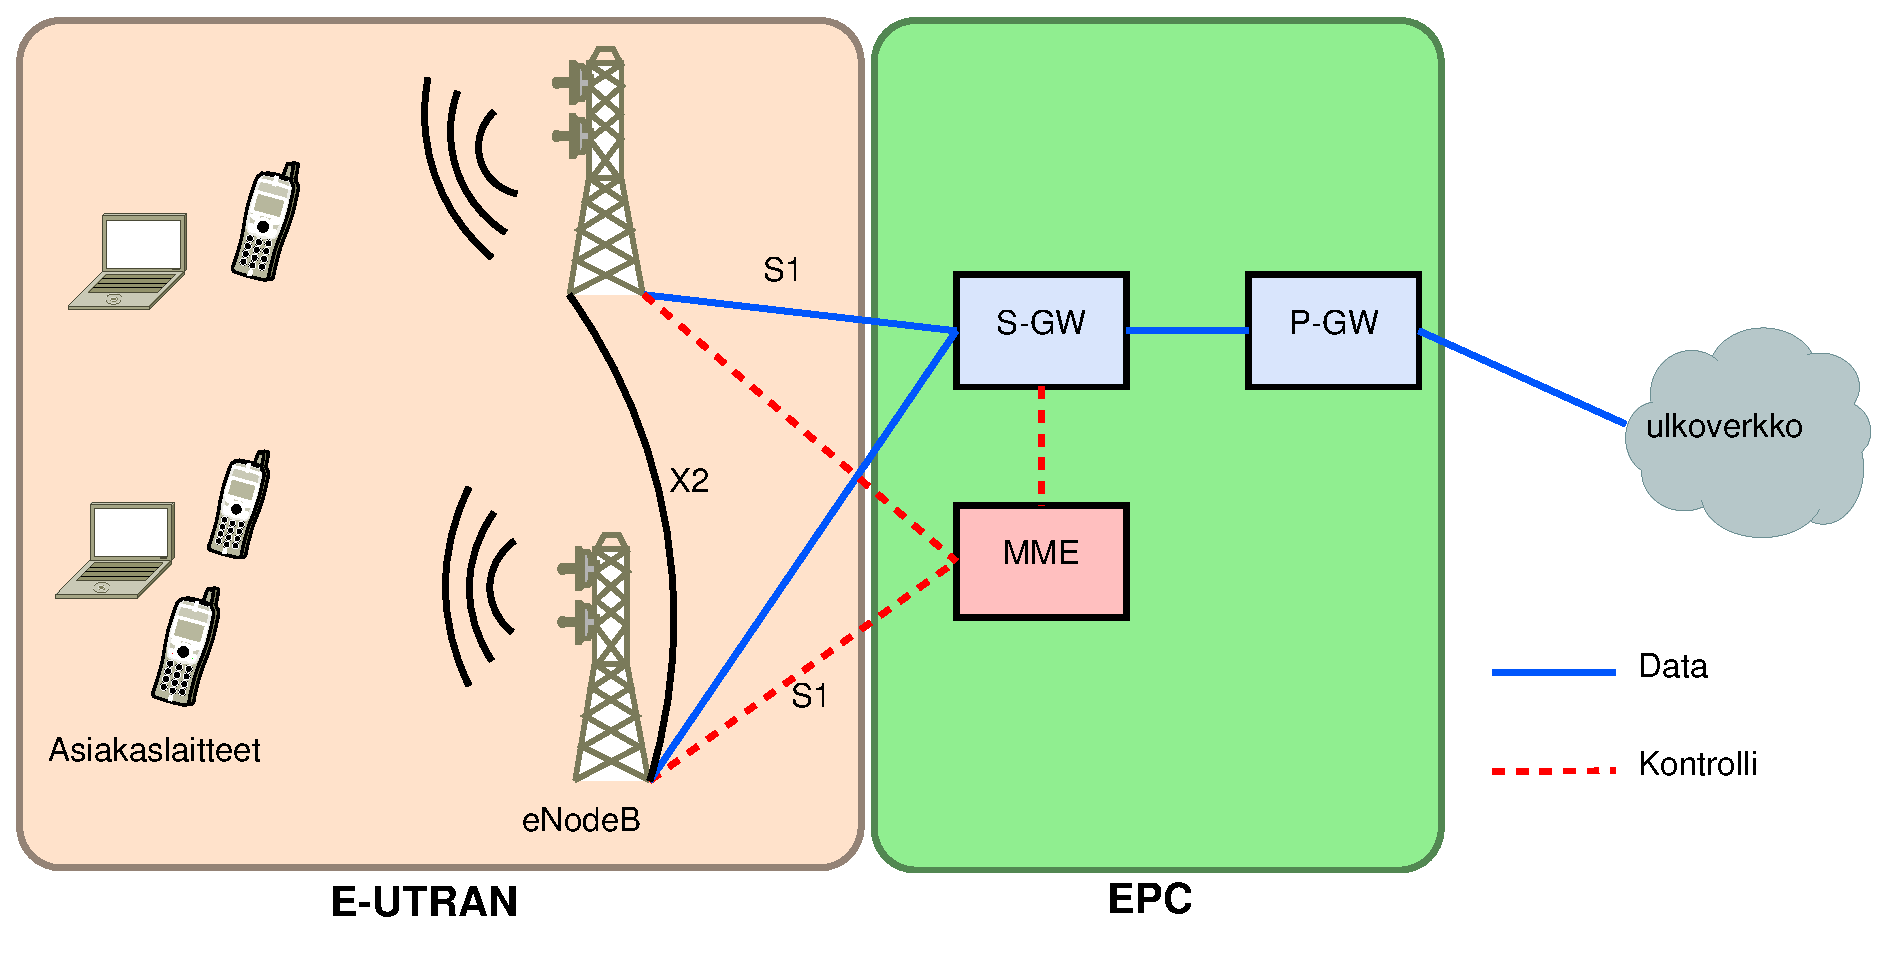
\includegraphics[width = \textwidth]{EPC.eps}
\caption{Yksinkertaistettu LTE-tyyppisen mobiiliverkon rakenne.} \label{fig:mobiarch}
\end{figure}

Tässä tutkielmassa käsiteltävät reuna-arkkitehtuurit sisältävät yhdistävänä tekijänä tavoitteen toimia mobiiliverkon yhteydessä. 
Täten reuna-arkkitehtuurien suunnittelupäätöksiä tarkasteltaessa on tarpeen ymmärtää mobiiliverkon osat yleisellä tasolla.
Yksinkertaisuuden vuoksi tämän tutkielman puitteissa mobiiliverkoksi oletetaan LTE:n mukainen arkkitehtuuri, joka koostuu E-UTRAN tyyppisestä radioverkosta ja EPC tyyppisestä runkoverkosta.
Seuraavaksi käydään läpi mobiiliverkon arkkitehtuurin tämän tutkielman kannalta merkitykselliset toimijat ja toiminnot.

Korkealla tasolla tarkasteltuna mobiiliverkko koostuu kahdesta osiosta: radioverkosta ja runkoverkosta. 3GPP kehittämässä LTE (Long Term Evolution) standardissa radioverkon sisältävä osuus on nimeltään E-UTRAN (Evolved UMTS Terrestrial Radio Access Network) ja runkoverkon osuus on nimeltään EPC (Evolved Packet Core).
E-UTRAN ja EPC väliset yhteydet on kuvattu kuvassa \ref{fig:mobiarch}.

E-UTRAN tehtävänä on toimia rajapintana asiakaslaitteen ja EPC:n välillä. 
E-UTRAN sisältää verkon puolella pääasiallisena toimijana eNodeB (Evolved nodeB) tyyppisiä tukiasemia \cite{etsieutran}.
Tukiasemista on olemassa muutamia erilaisia variaatioita, mutta tässä tutkielmassa käsitellään ainoastaan perustapausta.
Tukiasema on asiakaslaitetta lähimpänä sijaitseva funktionaalinen verkon osa ja sen seurauksena se on houkutteleva kohde reunalaskennan ratkaisuille. Tietoliikenteen näkökulmasta tukiaseman voi ajatella \textit{reunan} viimeisenä etappina ennen asiakaslaitteita. 

ENodeB tarjoaa asiakaslaitteiden suuntaan radioyhteyden.
EPC:n suuntaan eNodeB:t ovat yhteydessä S1 rajapinnan avulla.
Lisäksi eNodeB:t voivat olla toisiinsa yhteydessä X2 rajapinnan kautta.
S1:stä käytetään eNodeB:n ja EPC:n väliseen kommunikointiin. Tämä sisältää sekä hallinnollisen viestinnän, että asiakkaan tietoliikenteen kuljettamisen.
X2 rajapintaa puolestaan käytetään tukiasemien väliseen kommunikointiin. 
ENodeB välisten X2 yhteyksien tavoitteena on nopeuttaa tukiasemien välistä kommunikaatiota, esimerkiksi handoverin yhteydessä tehtävää asiakaskontekstin siirtoa varten \cite{3gpplte}.
Handoverilla tarkoitetaan asiakaslaitteen radioyhteyden siirtoa toiselle tukiasemalle. Handover käsitellään tarkemmin kappaleessa \ref{livemigraatio}.

Mobiiliverkon runkona toimiva EPC koostuu useista loogisista komponenteista.
Tämä siis tarkoittaa että toiminnallisuudet voivat fyysisesti sijaita samassa laitteessa. 
Tässä tutkielmassa on tarpeen ymmärtää perusteet seuraavista alikomponentista: MME (Mobility Management Entity), S-GW (Serving Gateway) ja PDN GW (P-GW, Packet data network gateway) \cite{etsilte}.
\begin{itemize}
\item \textbf{MME} on EPC:n hallinnollinen entiteetti joka vastaa muun muassa asiakaslaitteen tunnistamisesta ja handoveriin liittyvistä toimista EPC:n sisällä. Toisin kuin S-GW ja P-GW, MME ei käsittele asiakaslaitteiden tietoliikennettä.
\item \textbf{S-GW} eli palveluyhdyskäytävä toimii asiakaslaitteen EPC:n sisäisenä kiintopisteenä.  S-GW reitittää asiakaslaitteen liikennettä P-GW:n ja E-UTRAN välillä.
\item \textbf{P-GW} eli pakettiverkon yhdyskäytävän tehtävänä on toimia asiakaslaitteen ja mobiiliverkon ulkopuolisten IP-verkkojen yhteyspisteenä.
\end{itemize}
\cite{3gppepc}

Mobiiliverkossa käytävä kommunikaatio voidaan jakaa kahteen kerrokseen: kontrollikerrokseen ja tietoliikennekerrokseen.
Kontrollikerroksella välitettävät viestit ovat tarkoitettu hallinnollisiin toimintoihin mobiiliverkon sisällä. 
Tietoliikennekerros välittää asiakkaan tietoliikennettä internetin ja asiakaslaitteen välillä.
Asiakkaan tietoliikenne kulkee tukiaseman ja P-GW:n välillä GTP-tunneloituna (GPRS Tunnelling Protocol) \cite{puente15seamless}. Tämä tarkoittaa että mobiiliverkon sisällä tietoliikennettä ei ohjata asiakaslaitteen tietoliikenteen tunnisteiden pohjalta. 


\subsection{Reuna-arkkitehtuuri}
%Määrittele mikä on reuna-arkkitehtuuri


Tässä tutkielmassa käsiteltävät arkkitehtuurit ovat pääasiassa tyypiltään oletusarkkitehtuureja (framework). 
Tämänkaltaisen arkkitehturin tarkoituksena on jakaa järjestelmä toiminnallisiin osiin fyysisellä ja ohjelmallisella tasolla \cite{ohark}. Se siis kuvaa järjestelmän rakenneosien tehtävät.
Oletusarkkitehtuuria voidaan hyödyntää varsinaista toteutettavaa järjestelmää suunniteltaessa.

Kappaleessa \ref{reunatoimijat} kuvattujen reunan toimijoiden osalta reuna-arkkitehtuurit keskittyvät kuvaamaan reunasolmun ja reuna-alustan tehtäviä. Lisäksi reuna-arkkitehtuurit kuvaavat koko järjestelmän osana toista järjestelmää, jolloin reunajärjestelmä itsessään on komponentti suuremmassa järjestelmässä. Tällä tasolla tarkasteltu arkkitehtuuri jättää avoimeksi reunasovelluksien toiminnan ja keskittyy kuvaamaan reunasovelluksien sijaintia järjestelmässä.

Tämän tutkielman puitteissa arkkitehtuurilla tarkoitetaan reuna-alustan ja reunasolmujen muodostamaa järjestelmää. Reuna-alustan toiminnallisuuksia voisi eritellä vielä tarkemmin, etenkin reunasovelluksien hallinnan osalta. Cloudlet on konkreettinen toteutus reuna-alustan reunasovelluksia hallinnoivasta osasta, mutta se ei kata kuin yhden reunasolmun kerrallaan. 
Tämän lisäksi olemassa on reunasolmujen välisestä hallinnasta vastaava kerros, tosin tämä kerros voi olla ulkoistettu erillisille hallinnolliselle toimijalle, jolloin hallinnollinen osa reuna-alustasta on varsinaisten reunasolmujen ulkopuolella. 

Reunasovelluksien toimintaa ei käsitellä tarkemmin. Taxonomy paperissa on hyvä jaottelu erilaisista sovelluksista. Tämä aihepiiri laajenee sovelluksien jakamiseen osittain reunalla suoritettaviin (offloading) tai mobiilisovelluksen suoritusta tukeviin sovelluksiin. 



\section{Mahdollistavat teknologiat}
Seuraavaksi käsitellään reunalaskennan mahdollistavat teknologiat SDN, NFV ja virtualisointi. Tähän esiteltäväksi valittujen teknologioiden joukko perustuu tämän tutkielman luvussa \ref{ratkaisut} esitettyjen arkkitehtuuriratkaisujen yhteydessä esiintyneisiin teknologioihin.
Edellä mainittujen teknologioiden lisäksi reunalaskentaa käsittelevien julkaisujen yhteydessä on esitetty myös muita teknologioita kuten verkon viipalointi (network slicing) \cite{taleb2017multi}, jonka käsittely sivuutetaan tämän tutkielman yhteydessä.

\subsection{Virtuaalikoneet ja kontit}

%miten virtuaalikone toimii
Virtualisoinnilla tarkoitetaan tietokoneohjelmiston suorittamista ohjelmallisesti toteutetun rajapinnan päällä. 
Toisin sanoen virtualisointi erottaa suoritettan ohjelmiston suorittavasta laitteistosta.
Usein virtualisoitava ohjelmisto on kokonainen käyttöjärjestelmä, jolloin suoritettavaa instanssia kutsutaan virtuaalikoneeksi. 
Virtualisointi mahdollistaa laitteiston resurssien jakamisen useamman toisistaan erillään olevan virtuaalikoneen kesken.
Juurikin resurssien jakamisen mahdollisuus yhdessä palvelinlaitteiston suorituskyvyn kasvun kanssa on johtanut virtuaalikoneiden käytön yleistymiseen palvelinsaliympäristössä.

Virtuaalikoneen ja laitteiston välillä toimivaa ohjelmistoa kutsutaan hypervisoriksi. Hypervisorin pääasiallinen tehtävänä on tarjota rautatason resursseja virtuaalikoneiden käytettäväksi. 
Yksi hypervisorin tehtävistä on virtuaalikoneiden luominen. Sen avulla voidaan määrittä virtuaalikoneen käytössä olevat resurssit, esimerkiksi virtuaalikoneen käytettävissä olevan muistin tai prosessorien määrä. Hypervisorilla on myös monia muita toiminnallisuuksia, joita ei tässä tutkielmassa käydä läpi tämän enempää. 

%virtuaalikoneet reunalla
Virtuaalikoneet ovat vahvasti esillä reunalaskenta-arkkitehtuurien yhteydessä. 
ETSI:n reunalaskennan referenssiarkkitehtuurissa \cite{etsirefarch} virtuaalikoneet esitetään reunapalvelun tuottamisen välineenä ja Taleb et al. \cite{taleb2017multi} esittävät kirjallisuuskatsauksessaan virtuaalikoneet yhdeksi reunalaskennan mahdollistavista teknologioista.
Virtuaalikoneiden dynaamisuus verrattuna tavallisesti suoritettavaan ohjelmistoon on reunalaskennan näkökulmsta haluttu ominaisuus. 
Virtuaalikoneet tarjoavat myös helpon tavan jakaa reunasolmun resursseja usean toisistaan erillisen palvelun välillä.
Toisena etuna on virtuaalikoneiden vahva eristys muusta järjestelmästä ja muista virtuaalikoneista.

Virtuaalikoneet eivät aseta rajoitteita tarjottavan palvelun tyypille ja niiden avulla onkin mahdollista tarjota monia erilaisia palvelumalleja.
Yksi ehdotetuista palvelumalleista on käyttäjäkohtaisen virtuaalikoneet \cite{satya09,wang2015mobiscud}. 

%mitä se mahdollistaa
Tulevissa kappaleissa perehdytään tarkemmin virtuaalikoneiden hyödyntämistä osana reunapalveluita.
Kappaleessa \ref{livemigraatio} käsittellään virtuaalikoneiden siirtelyä suorituslaitteistolta toiselle, ilman että itse järjestelmän suorittamista tarvitsee keskeyttää siirron ajaksi. 
Kappaleessa \ref{cloudlet} käsitellään cloudletiksi nimettyä  virtuaalikoneisiin pohjautuvaa reunapalvelun tuottamisjärjestelmää.




\subsection{Software-defined networking}
Perinteinen tietoliikenneverkko koostuu joukosta erikoistuneista verkkolaitteita. 
Tällaisia laitteita ovat esimerkiksi kytkin, palomuuri ja reititin. Näiden laitteiden joukko muodostaa hajautetun rakenteen, jossa jokainen laite täytyy konfiguroida erikseen.
Laitevalmistajat tarjoavat hallinnointityökaluja, joiden avulla valmistajan omia laitteita on mahdollista konfiguroida suljettua rajapintaa käyttäen. Verkkoinfrastruktuurin hallintaa kuitenkin vaikeuttaa eri laitteiden konfiguraatioiden erilaisuus, sekä puute kokonaisvaltaiselle ohjelmalliselle konfiguroitavuudelle.
Tästä johtuen verkkoon tehtävät muutokset ovat työläitä ja riskialttiita \cite{kreutz2015software}.

Perinteisessä tietoliikennelaitteistossa tiedonvälityskerros ja kontrollikerros ovat tiukasti toisistaan riippuvaisia. Tiedonvälityskerroksella tarkoitetaan itse tietoliikennepakettien välittämiseen käytettävää kerrosta, eli tietoliikennettä ohjaavia laitteistoja. Kontrollikerroksella tarkoitetaan tietoliikenteen reitittämiseksi käytettävää logiikkaa, kuten esimerkiksi reititystauluja. Kontrollikerros on siis tällä hetkellä hajautettuna laitteiston mukana ympäri verkkoa. Tästä johtuen verkko on usein hyvin staattinen ja muutokset kankeita.

SDN (Software-defined networking) eli ohjelmallisesti määritetty verkko on yleistyvä paradigma verkkoympäristöissä.  SDN on ratkaisu, jossa tiedonvälitys- ja kontrollikerros on erotettu toisistaan. SDN:ssä ei ole erikoistunutta verkkolaitteistoa vaan nykyinen tiedonvälitykseen käytetty laitteisto korvattaisiin yleisillä reitittävillä laitteilla\footnote{Reitittämisellä tarkoitetaan tässä yhteydessä pakettien ohjausta ja välitystä yleisessä mielessä}. Kontrollikerroksen toiminnasta vastaa SDN Controller. Se on loogisesti keskitetty entiteetti, joka vastaa näiden reitittävien laitteiden ohjaamisesta.

SDN Controllerin ja reitittävän laitteiston välille oletetaan hyvin määritelty rajapinta, jonka kautta reitittäviä laitteita voidaan hallita \cite{kreutz2015software}. SDN siis toteuttaa \textit{Separation of Concerns} -periaatetta jakamalla verkon reititysmäärittelyjen konfiguroinnin ja itse laitteistopohjaisen toteutuksen omiin osiinsa. SDN Controller tarjoaa rajapinnan ylöspäin ohjelmalliselle verkkokonfiguroinnille ja hoitaa sääntöjen tulkkaamisen alaspäin. OpenFlow on yksi tunnetuimmista SDN Controllerin ja verkkolaitteiden välisestä protokollasta\footnote{\url{https://www.opennetworking.org/software-defined-standards/specifications/}}.

% TODO Flow sääntöjen toiminta.

Tarve SDN pohjaisille ratkaisuille kumpuaa jo aiemmin mainitusta konfiguraation työläydestä ja dynaamisuuden tarpeesta. Esimerkiksi virtuaalikoneiden käytön yleistyessä tarve verkon ohjelmalliselle hallittavuudelle on kasvanut \cite{jammal2014software}. Virtuaalikoneiden sijainti verkossa ei välttämättä ole kiinteä, vaan virtuaalikone saattaa siirtyä esimerkiksi migratoinnin seurauksena. Virtuaalikoneita saattaa tulla ja poistua verkosta. Perinteisessä verkkoympäristössä esimerkiksi MAC osoitetaulujen päivittäminen saattaa aiheuttaa yhteyskatkoksia palvelimeen \cite{jammal2014software}. SDN pohjaisia ratkaisuja on jo olemassa, mutta niiden käyttö ei vielä ole korvannut perinteisiä verkkolaitteita. 


\subsection{Network function virtualization} \label{nfv}
NFV (Network function virtualization) lähtee liikkeelle ongelmasta, jossa nykyisen verkkolaitteiston käyttöikä on lyhyttä ja toiminnot ovat hajautettuina useisiin suljettuihin (proprietary) laitteisiin \cite{nfvwhite}. 

NFV:n tarkoituksena on eriyttää verkkolaitteisto ja verkkotoiminnot. Tämä toteutuisi siten, että erillistä verkkolaitteistoa ei enää tarvittaisi ja nykyisten verkkolaitteiden toiminnallisuudet toteutettaisiin tavallisella palvelinlaitteistolla ohjelmatasolla. Periaate on hyvin samankaltainen kuin perinteisten palvelimien siirtyminen virtuaalikoneita hyödyntävään ympäristöön.
Virtualisoidulla verkkotoiminnallisuudella (jossain yhteyksissä VNF, Virtualized network function) tarkoitetaan ohjelmallisesti toteutettua verkkotoimintoa. Tämä mahdollistaa verkkotoiminnallisuuksien suorittamisen tavallisella palvelinlaitteistoilla hyprvisorin päällä. 

Verkkotoimintojen toteuttaminen virtuaalisina, mahdollistaisi useamman toiminnon sijoittamisen samaan laitteistoon. Tämä ainakin teoriassa mahdollistaisi myös paremman skaalautuvuuden. Myös verkkotoiminnallisuuksien käyttöönotto helpottuu mikäli erillisen laitteiston asennusta ei tarvita. Virtuaalisten verkkotoimintojen avulla on myös mahdollista säästää kaappitilaa sekä pienentää sähkönkulutusta \cite{nfvedge}.

NFV on soveltuva mille tahansa datatason (data plane) prosessoinnille ja kontrollitason (control plane) toiminnoille \cite{nfvwhite}. NFV siis soveltuu toteutustavaksi monille erilaisille verkkoitoiminnoille mobiiliverkoissa ja perinteisissä tietoliikenneverkoissa. Esimerkkeinä käyttökohteista ETSI:n NFV white paperissä on esitetty muun muassa reitittimet, palomuurit, kuormantasaajat, eNodeB:t ja MME:t. ETSI on pohtinut NFV:n laajamittaisen käyttöönoton mahdollisuuksia 5G-verkkoingrastruktuurissa ja mainitsee reunalaskennan yhtenä sen käyttötapauksena \cite{etsinfv5g}.

Yksi NFV:hen pohjautuvista ideoista on C-RAN (Cloud radio acceess network), joka pyrkii virtualisoimaan tukiaseman toinnot \cite{chih2014recent}. Käytännössä tukiaseman fyysiseen sijaintiin vietäisiin kuituyhteys ja RRU (Remote radio unit).
RRU sisältäisi radiosignalointiin tarvittavan laitteiston sekä laitteiston, joka muuttaa radion ja kuituyhteyden välillä olevaa tietoliikennettä analogisen ja digitaalisen muodon välillä.
Kuituyhteys välittää signaalin ohjelmallisesti toteutetulle BBU:lle (Baseband Unit), joka hoitaa kaikki tukiaseman toiminnot \cite{chih2014recent}.
BBU:t voitaisiin virtualisoida ja suorittaa keskitetysti palvelinsaleissa.
Toistaiseksi tukiaseman resurssit on mitoitettu suurimman mahdollisen kuorman mukaan. Virtualisoinnin avulla BBU:n resurssit olisivat paremmin skaalattavissa.
Kappaleessa \ref{concert} esitellään reuna-arkkitehtuuri, joka rakentuu C-RAN tyyliseen verkkoon.

Mobiiliverkossa toimivan reunalaskennan näkökulmasta NFV:n potentiaali on ilmeinen. Jos suurin osa mobiiliverkon toiminnoista voitaisiin virtualisoida ja siirtää tavalliselle palvelinlaitteistolle, voisi reunalaskentaa suorittaa samalla laitteistolla, eikä se vaatisi erillistä laitteistoa omille toiminnoilleen.
NFV:n haasteena on toteutuksien puute. 


\section{Ominaisuudet}

Reunalaskennan keskeisin tarkoitus on laskennan siirtäminen reunalla toimivalle reunalaskentaklusterille. Reunaa voidaan lähestyä pilven ja käyttäjälaitteiden puolelta. Käyttäjälaitteiden, kuten älypuhelimien laskentateho on suhteellisen heikkoa, lisäksi ne ovat akkuvirrasta riippuvaisia. 
Mobiililaitteen käyttöajan pidentämiseksi voidaan pyrkiä tekemään mahdollisimman vähän akkuakuluttavaa laskentaa paikallisesti, siirtämällä sitä reunalaskentaklusterille (Etsi se lähde jossa verrataan tietokoneita ja mobiililaitteita - eroa oli yhden kertaluokan verran).
Esimerkiksi verkkoliikenne mobiililaitteen ja kohdepalvelimen välillä on merkittävä viive toisi reunaklusteri palvelun huomattavasti lähemmäksi ja pienentäisi viivettä palvelussa. Viiveen pienenemisen seurauksena monet reaaliaikaisuuttaa tai nopeaa reagointia vaativat palvelut ovat mahdollisia. Lisäksi verkon viiveestä tai ruuhkasta johtuen, mobiililaitteella on usein huomattavasti nopeampi yhteys fyysisesti lähelle itseään verra

Lisäksi pilven tai konesalien suunnasta asiaa lähestyttäessä runkoverkko tukkeutuu. Siirtämällä osan palveluvastuusta reunalle, runkoverkon rasitteen tulisi ainakin periaatteessa pienentyä. 

\subsection{Kommunikaatio}
Reunan keskeisin haaste kommunikaatiossa on asiakaslaitteen ja reunasolmun välisen kommunikaation ylläpitäminen.

\subsection{Etälaskenta}
Etälaskennan toteuttamiseksi tarvitaan vastaukset seuraaviin kysymyksiin. Mitä siirretään ja minne siirretään?

MOCAssa oli selitetty kuinka muodostetaan yhteys in-network cloudiin.

Etälaskenta voidaan karkeasti jakaa kahteen tyyppiin: Binääriseen ja osittaiseen \cite{mao17}. \textit{Onkohan ok lainata surveytä?}. Binäärisessä ohjelmasta suoritetaan selkeitä kokonaisuuksia joko reunasolmulla tai asiakaslaitteella. Osittaisessa etälaskennassa suoritusta siirretään dynaamisesti reunasolmulle. 

Offloading on varmaan samankaltainen termi.
Reunalla suoritettava etälaskenta saattaa siirtää ohjelman suorituksen kokonaan tai osittain asiakaslaitteelta reunasolmulle. Laskennan tulos lähetetään takaisin asiakaslaitteelle ja sitä käytetään osana muuta laskentaa. 
Laskennan hallinta suoritetaan asiakaslaitteella. Etälaskentaa motivoi raskaiden operaatioiden siirtäminen asiakaslaitteelta reunalle. Erityisesti mobiililaitteilla akkuvirran säästäminen on keskinen tekijä. Etälaskennan kannattavuus puhtaasti akkuvirran näkökulmasta muuttuu kannattavaksi, kun suoritettavan ohjelman lähettäminen ja tuloksen vastaanottaminen kuluttavat vähemmän akkua kuin ohjelman suorittaminen paikallisesti asiakaslaitteella.
Todellisuudessa pelkästään akkuvirran säästäminen ei riitä, sillä muuten laskentaa voitaisiin siirtää pilveen. QoS kuitenkin heikkenee, mikäli laskennan suorittamiseen kuluva aika pitenee huomattavasti.
Reunalle on teoriassa nopeampi yhteys ja nopeampi vastaus. Voitaisiin siis laskea että suoritusajassa mitaten ohjelman siirtäminen reunalle on kannattavaa kun suoritettavan ohjelman lähettäminen palvelimelle, sen suorittaminen ja tuloksen vastaanottaminen kestävät vähemmän aikaa kuin ohjelman suorittaminen paikallisesti. 
Ongelmana on että suorituksien aikavaatimus ei ole eksakti vaan ainoastaan arivoitavissa. Lisäksi suoritusaikainen aika-arvion tekeminen vie myös aikaa. 
Ajan ja akkuvirran säästämiseksi tehtävät toimet ovat siis keskeisimmät haasteet etälaskentaa toteutettaessa. Näiden käsittelyä ei tämän enempää tässä tutkielmassa käsitellä niiden monimutkaisuuden vuoksi.


%\subsection{Etäinstanssi}
%Etäinstanssissa asiakaslaitteella on yhteys reunalle. Asiakaslaitteelle tulee ainoastaan näkymä palvelun tilasta omalle laitteelleen. Vastaavasti kuin ottaisi SSH tai VNC yhteyden toiselle laitteelle. 

\subsection{Live migraatio} \label{livemigraatio}

%Alkukappale
%% Mitä migraatio on ja miten se liittyy handoveriin
Live migraatio, eli suorituksen aikanen siirto, tarkoittaa virtualisoidun ohjelman tai virtuaalikoneen siirtämistä laitteistolta toiselle, siten että virtuaalikoneen käyttö ei keskeydy siirron ajaksi \cite{clark2005live}. 
Useimmiten tällaista toiminnallisuutta käytetään palvelinkeskuksissa virtuaalikoneiden
siirtelyyn. Palvelinkeskuksissa siirtämiseen käytetään nopeita sisäisiä yhteyksiä,
jolloin tiedon siirtoon käytettävät väylät ovat nopeita. Syitä live migraation
suorittamiseksi on muutamia. Perinteisessä palvelinympäristössä live migraation
syinä ovat virrankulutuksen optimointi, kuorman tasaaminen tai fyysisen
laitteiston huoltoon ottaminen \cite{soni2013comparative}. 

Reunalaskentaan sovellettuna live migraation tehtävänä on laskentaa tai palvelua suorittavan virtuaalikoneen siirtäminen reunasolmujen välillä.
Syyt joiden vuoksi reunalaskentaympäristössä tehdään live migraatiota koskevat pääasiassa asiakaslaitteen liikkumista verkossa, jolloin virtuaalikone siirretään asiakaslaitetta lähimpänä olevalle  reunasolmulle. 
Reunalaskentaa suoritettaessa voi myös tulla tilanne, jossa laskentaa suorittavalla reunasolmulla ei ole resursseja laskennan suorittamiseksi. Tällöin asiakkaan virtuaalikone saatetaan joutua joudutaan siirtämään toiselle reunasolmulle, jolla on enemmän resursseja.  


\subsubsection*{Handover/handoff}%omaan kappaleeseensa?
Virtuaalikoneille tehtävän live migraation ja mobiiliverkossa suoritettavan handoverin ideat ovat samankaltaisia. Molemmissa tavoitteena asiakasta palvelevan entiteetin siirtäminen ilman että asiakas huomaa siirtoa.
Handoverilla tarkoitetaan asiakaslaitteen radioyhteyden siirtämistä tukiasemalta toiselle tukiasemalle. 
LTE:ssä handover päätös tehdään eNodeB:ssä asiakaslaitteen välittämän mittaustuloksen perusteella. 
Handover voidaan tehdä esimerkiksi tilanteessa jossa asiakaslaitteen ympäristössä on toinen tukiasema, joka voisi palvella asiakaslaitetta paremmin \cite[s.~96]{etsilte}.
LTE:ssä yhteys on tyypiltään tunnelimainen ja handoverissa tunnelin toinen pää siirretään toiselle tukiasemalle.
Yhteyden siirron alkaessa tukiasema välittää kohteena olevalle tukiasemalle asiakaslaitetta koskevat tilatiedot. Kun tilatiedot on välitetty, asiakaslaitteen ja tukiaseman välinen yhteys katkaistaan ja asiakaslaite muodostaa yhteyden uudelle tukiasemalle.
Asiakaslaitteen tietoliikennettä puskuroidaan S-GW:n toimesta sillä välin kun yhteys on katkaistuna. Yleensä handover on niin nopea toimenpide, että laitteen käyttäjä ei sitä huomaa.
Handover on nopea toimenpide koska sen aikana siirrettävän tiedon määrä on vähäinen.
Handoverin sisältämä asiakaskonteksti koostuu pääasiassa erilaisista asiakaslaitteen ja tunneleiden tunnisteista.

\subsubsection*{Live migraation toiminta}%Miten migraatio toimii
Live migraatiossa virtuaalikone siirretään palvelimelta toiselle palvelimelle, ilman että virtuaalikoneen käyttö keskeytyy. 
Perinteinen live migraatio on toteutettu siten, että virtuaalikoneen suoritustilan eli prosessorin tilan ja muistin siirretään toiselle palvelimelle.

Siirtäminen suoritetaan iteraatioittan siten, että ensimmäisellä iteraatiolla kaikki muistisivut siirretään kohdelaitteelle \cite{clark2005live}.
Seuraavilla kierroksilla lähtölaitteelta siirretään vain ne muistisivut joille on tapahtunut muutoksia edellisen siirron alkamisen jälkeen. 
Tätä jatketaan kunnes muutoksia sisältävien muistisivujen määrä ei vähene iteraatioittan.
Tässä vaiheessa lähtöpisteenä oleva virtuaalikone pysäytetään ja loput virtuaalikoneen muistisivut ja tilatiedot siirretään kohdelaitteelle. Tämän jälkeen virtuaalikone käynnistetään uudessa sijainnissa. 

Live migraatioon liittyy myös erilaisia optimointeja ja lähestymistapoja, joita ei tässä tutkielmassa sen tarkemmin avata. 
Palvelinsaliympäristössä on myös yleistä, että virtuaalikoneen tallennustilaa ei ole tarpeen siirtää, koska se on toteutettu levypalvelimen avulla, jolloin ainoastaan yhteys täytyy siirtää \cite{clark2005live}. Mikäli näin ei ole, myös tallennustila tulee siirtää laitteelta toiselle.
Live migraatio vaatii myös avoimina olleiden tietoliikenneyhteyksien siirtämisen \cite{clark2005live}.

Live migraation suorituskykyä mitataan seuraavilla metriikoilla \cite{soni2013comparative}:

\begin{itemize}
	\item Migraation kesto: Aika joka kuluu migraation suorittamiseen
	\item Katkon kesto: Aika jona palvelut eivät käytettävissä
	\item Siirretyn datan määrä: Migraatiosta aiheutuva tietoliikenteen määrä
	\item Migraation yleisrasite: Paljonko migraatio vie järjestelmän resursseja
	\item Suorituskyvyn alentuma: Siirrettävän virtuaalikoneen suorituskyvyn heikentyminen siirron aikana
\end{itemize}

Näistä kolme ensimmäistä ovat keskeisimpiä \cite{farris2017lightweight}. Tavoitteena perinteisessä live migraatiossa on mahdollisimman lyhyt käyttökatko \cite{ha2015adaptive}.

%Migraation uudethaasteet reunalla vs palvelinsali
\subsubsection*{Reunalaskennassa}
Reunalaskentaympäristössä suoritettavan live migraation toiminnallisuus on pääpiirteittäin sama kuin edellä kuvattu.
Reunalaskennassa live migraatiolla viitataan reunasovelluksen suoritusaikaiseen siirtoon reunasolmujen välillä.
Live migraation tavoitteena on taata asiakaslaitteen parempi palvelu.
Keinona tuon tavoitteen saavuttamiseksi on esimerkiksi reunasovelluksen siirtäminen asiakasta lähempänä sijaitsevalle reunasolmulle. Reunalla tehtävän live migraation erona palvelinsaliympäristöön on juurikin suoritusympäristö. 

Päällimmäisenä erona on palvelinsaleissa tehtävään migraatioon on käytettävien yhteyksien nopeus. Reunasolmujen väliset yhteydet ovat oletettavasti hitaampia ja nopeus saattaa vaihdella\cite{ha2017you}.
Hitaat yhteyden johtavat pitkään siirtoaikaan, joka puolestaa johtaa pidempään käyttökatkokseen ja täten palvelun laadun heikkenemiseen. 
Reunajärjestelmissä ei myöskään oletettavasti ole jaettua levyplalvelinta, vaan reunalaskennan yhteydessä live migraatio sisältää myös massamuistin siirron.

Esimerkkitilanteessa jossa asiakaslaite on siirtynyt alkuperäisen reunasolmun kantaman ulkopuolelle reunasovelluksen käyttö voi jatkua reititysmuutoksen avulla. Asiakaslaitteen siirtyessä kauemmaksi alkuperäisestä reunasolmusta, viiveet kasvavat ja palvelun laatu heikkenee. Reunajärjestelmä aloittaa asiakasta palvelevan reunasovelluksen migraation lähempänä sijaitsevalle reunasolmulle.
Huomion arvoinen seikka on että asiakkaan palvelun laatu pysyy heikentyneenä niin kauan kuin live migraatio on käynnissä ja alkuperäisen reunasolmun edelleen palvellessa asiakasta. 
Toisin sanoen reunalaskennassa live migraation kannalta on tärkeää minimoida live migraatioon kuluva kokonaisaika. 
Kokonaisajan minimoimiseksi joudutaan todennäköisimmin luistamaan katkoksen kestosta. 
Etenkin hitailla yhteyksillä tiedon siirtoon kuluva aika on kertaluokkaa suurempi kuin katkoksen kesto \cite{ha2017you}.
Siirtoajan minimoimiseksi on pyrittävä pitämään siirrettävän datan määrä mahdollisimman pienenä \cite{ha2015adaptive}.



% Tämän lisäksi reunasolmuilla ei ole nykyisten ratkaisuehdotusten mukaan käyttössään yhteistä levypalvelinta, eli myös tallennustila joudutaan muodossa tai toisessa siirtämään live migraation yhteydessä. 


Palvelinsaleja ja reunalaskentaympäristöä erottaa myös se, että palvelinsaliympäristössä virtuaalikoneiden live migraatiot voidaan pääsääntöisesti tehdä koordinoidusti ilman tiukkkoja aikarajoitteita. 
Reunalaskentaympäristössä migraatiopäätös perustuu usein johonkin ulkoiseen tapahtumaan. Todennäköisintä onkin että migraatiopäätös tehdään samankalataisin perustein kuin edellä esitellyn handoverin. Keskeisin syy migraatiolle oletettavasti on asiakaslaitteen liikkuminen verkossa, mutta syynä voi olla myös esimerkiksi reunasolmun ruuhkautuminen. Asiakaslaitteiden liikkumiseen pohjautuva migraatio yhdistettynä heikkoihin tietoliikenneyhteyksiin on kuitenkin ongelmallinen. Voidaan esimerkiksi kuvitella tilanne jossa aamulla kaupungin keskustaan saapuvat työmatkailijat aiheuttavat "migraatiotulvan". Suuri määrä migraatioita saattaa ruuhkauttaa reunasolmujen käytössä olevat tietoliikenneyhteydet ja käyttää suuren osan käytössä olevista resursseista. 


%ratkaisuja
%ratkaisuja cloudlet
Lähes kaikki läpikäydyt reunalaskenta-arkkitehtuurit tiedostivat tarpeen reunasovelluksien migraatiolle, mutta kovin harvassa määriteltiin täsmällisiä toimia sen toteuttamiseksi.
Cloudlettien ympärillä tehdyn tutkimuksen yhteydessä on esitetty migraatioratkaisua, joka lyhentäisi migraation kestoa merkittävästi. Cloudlet ratkaisu käsitellään tarkemmin kappaleessa \ref{vmhandoff}. 
Onkin realistista olettaa, että varsinaiseen reunajärjestelmään toteutettava live migraatio toiminnallisuus optimoitaisiin reunaympäristöön sopivaksi, kuten cloudlettien yhteydessä on pyritty tekemään. 
%MobiScud:n yhteydessä käytettiin Xen hyperviisorin migraatiotoiminnallisuutta suoraan sovellettuna reunalaskentaympäristöön\cite{wang2015mobiscud}.

\subsection{Integraatio mobiiliverkkoihin}
\begin{quote}
Tarkista onko käsitelty myös niin että laitteistovaatimukset tulevat esiin. Esimerkiksi vaatiiko reunalaskennan toteuttaminen erikoisvalmisteisia laitteita vai selvitäänkö tavallisilla palvelimilla?
\end{quote}


Useat reunalaskentaan liittyvät arkkitehtuurit on suunniteltu integroitaviksi osaksi mobiiliverkkoa.
Motivaatio on ilmeinen, koska lähes kaikki mobiiliverkossa toimivat laitteet kuuluvat reunalaskennan kohderyhmään.
Reunalaskentatoiminnallisuutta lisättäessä olemassa olevaan järjestelmään, yhdeksi suurimmista tekijöistä tulee hinta. 
Kuten aiemmin mainittu, mobiiliverkon laitteisto on usein suljettu, eikä siihen välttämättä ole mahdollista tehdä muutoksia tai laajennoksia.
Tämä tarkoittaa että ainakin osa olemassa olevasta laitteistosta jouduttaisiin korvaamaan uudella, mikäli reunalaskentatoiminnallisuus halutaan lisätä.
Tämän vuoksi on esitetty tekniikoita joiden avulla laitteiston uusimiselta voidaan välttyä, tai ainakin minimoida korvattavan laitteiston määrä.
Yksi erottavata tekijä on reunalaskentaratkaisun sidonnaisuus mobiiliverkkoon. Tämä tarkoittaa että löyhästi sidonnaisten ratkaisujen tuottajana voi jokin kolmas osapuoli, mutta yleisesti tämä myös tarkoittaa että reunapalvelu tuotetaan kauempana reunasta.
Jokaisessa ratkaisussa on siis hyvät ja huonot puolensa. 

%Tavat joilla reunalaskenta voidaan lisätä osaksi mobiiliverkkoa voidaan jakaa kolmeen pääryhmään
Reunajärjestelmien tapa integroitua osaksi mobiiliverkkoa on jaettu tässä tutkielmassa kolmeen eri pääryhmään

\begin{itemize}
\item \textbf{Suorat integraatiot} sisältävät uusien toimintojen lisäämistä osaksi olemassa olevaa arkkitehtuuria. Tämänkaltainen ratkaisu edellyttää muutoksia myös olemassa olevien komponenttien toimintaan. 
\item \textbf{Epäsuorat itegraatiot} eivät edellytä toiminnallisia muutoksia mobiiliverkon toimintoihin.
\item \textbf{Läpinäkyvät integraatiot} vaativat muutoksia mobiiliverkkoon, mutta eivät vaadi muutoksia olemassa olevien komponenttien toimintaan.
\end{itemize}

Suorat integraatiot edustavat niiden ratkaisujen joukkoa jotka muokkaavat olemassa olevan mobiiliverkkoarkkitehtuuria.
Näiden ratkaisujen voidaan olettaa olevan kalleimpia, koska yhteistoiminnallisten toimijoiden lisääminen olemassa olevaan infrastruktuuriin vaatii muidenkin toimijoiden päivittämistä.
Pääasiassa nämä ratkaisut tähtäävät lisäämään reunalaskentaa viidennen generaation mobiiliverkkoihin, mutta myös LTE:hen pohjautuvia ratkaisuja on esitetty.
Koska viidennen generaation määrittelytyö on vielä kesken, ehdotetut ratkaisut rakentuvat osittain oletuksien päälle.
Esimerkkinä suorasta integraatiosta on CONCERT (esitellään kappaleessa \ref{concert}). Suora integraatio mahdollistaa reunalaskennan tuomisen niin lähelle reunaa kuin mahdollista.

Epäsuoralla integraatiolla tarkoitetaan ratkaisuja, joiden pääasiallinen toiminnallisuus on sijoitetu mobiiliverkko-arkkitehtuurin ulkopuolelle. 
Tällaiset ratkaisut mahdollistavat reunalaskentainfrastruktuurin tuottamisen kolmansilla osapuolilla. Esimerkkinä tällaisesta ratkaisusta on FMC (käsitellään tarkemmin kappaleessa \ref{fmc}). Haasteena tämänkaltaisissa ratkaisuissa on optimaalisen reunasolmun valinta, koska se joudutaan tekemään asiakaslaitteen antamien tietojen pohjalta. Onkin siis huomattava, että asiakaslaite joutuu osallistumaan reunalaskentaan liittyviin hallinnollisiin toimiin.

Läpinäkyvissä ratkaisuissa reunalaskennan mahdollistavat toiminnot on toteutettu siten että suoria yhteyksia mobiiliverkon toimintoihin ei ole. 
Periaate on hieman samankaltainen kuin läpinäkyvässä välipalvelimessa.
Käytännössä tämä tarkoittaa jonkinlaiseen tietoliikennemonitoriin pohjautuvaa ratkaisua. 
Monitorin tehtävänä on tarkkailla mobiiliverkon tapahtumia, sekä mahdollistaa halutun tietoliikenteen ohjaaminen reunalaskennalle.
Näiden toimintojen toteuttamisen helpottamiseksi käytössä on tai käyttöön oletetaan SDN, NFV tai molemmat.
Joskaan läpinäkyvät ratkaisut eivät ole osa mobiiliverkkoa, ne sijaitsevat sen välittömässä yhteydessä. Tämä sitoo ne osaksi mobiiliverkon infrastruktuuria ja käytännössä tämä tarkoittaa että reunapalvelualustan tuottajana on mobiiliverkon-operaattori. 
Esimerkkinä tällaisesta ratkaisusta on MobiScud, joka käydään tarkemmin läpi kappaleessa \ref{mobiscud}. Tämänkaltaiset ratkaisut ovat asiakaslaitteen näkökulmasta "näkymättömiä".


\subsection{Hallinta}

%Reunalaskenta-arkkitehtuurissa hallinnalla tarkoitetaan sellaisia toimia, jotka mahdollistavat, ylläpitävät ja säätelevät asiakaslaitteen ja reunasolmun välistä kommunikaatiota. Hallinnosta vastaavana entiteetin tai entiteettien keskeinen tehtävä on erilaisiin tapahtumiin reagoiminen. Yleisimmin arkkitehtuurien yhteydessä käsiteltävät tapahtumat ovat reunalaskennan aloittaminen, laskennan migraatio ja kommunikaatioväylän avaaminen. Tämän lisäksi hallinnollisiin toimiin oletetaan reunalaskennan resurssien varaaminen sekä niiden optimointi. Näitä ei kuitenkaan korkealla arkkitehtuuritasolla kuvata.


%%%%%%%%%%%%%%%%%%%%%%%

%Reunan hallinta
%Mitä tarkoitetaan hallinnalla?
Reunajärjestelmän hallinta koostuu joukosta reunajärjestelmän toimintaa sääteleviä entiteettejä. 
Tutkielmassa käsiteltävistä reunalaskenta-arkkitehtuureista identifioitiin päävastuussa oleva hallinnollinen toimija sekä joitakin hallinnollisia toimintoja.
Edellä kuvattu live migraation laukaiseminen ja kommunikaatioväylän muodostaminen olivat keskeisimmät tunnistetut hallinnolliset toiminnot.
Näiden toimien perusperiaate on, että hallinnollinen toimija saa herätteen jostain mobiiliverkon tapahtumasta ja välittää tarvittavat toimenpiteet reunasolmuilla sijaitsevalle reuna-alustalle. 

%Reunan hallinta koostuu joukosta hallinnollisia toimia toteuttavia entiteettejä.
%Tämän tutkielman yhteydessä hallinnolliset toimet rajautuvat pääasiassa niihin toimintoihin, jotka mahdollistavat, ylläpitävät tai säätelevät asiakaslaitteen ja reunasolmun välistä kommunikaatiota. 
%Arkkitehtuuritasolla keskeisimmät hallinnolliset toimijat liittyvätkin juuri reunasolmujen saavutettavuuden varmistamiseen.
%Tämän tutkielman esittelyjen ulkopuolelle jäävät siis ne hallinnolliset toimijat, jotka esiintyvät arkkitehtuurikuvauksissa pääasiassa mainintana. Esimerkiksi virtuaalikoneisiin pohjautuvien järjestelmien resurssien oikeanlainen utilisointi \cite{yousaf16fine, taleb2017multi} on keskeinen haaste reunalaskennassa, mutta arkkitehtuuritasolla siihen ei oteta juurikaan kantaa ja sen suunnittelu jätetään järjestelmän toteuttajan vastuulle.


Pääasiassa hallinnollisten toimijoiden rooli esiintyy reunalaskenta-arkkitehtuurissa passiivisena tarkkailijana, jonka tehtävä on reagoida mobiiliverkon tapahtumiin. 
Esimerkki tällaisesta tapahtumasta on mobiiliverkossa tapahtuva handover, johon hallinnollinen entiteetti saattaa haluta reagoida esimerkiksi aloittamalla reunalaskennan migraation lähemmäksi käyttäjää. 
Myös aktiivisten hallinnollisten toimijoiden tarve tiedostetaan, mutta tällä arkkitehtuuritasolla niitä ei määritellä.
Aktiivisten hallinnollisten suunnittelu jätetään reunajärjestelmän toteuttajalle.
Aktiivisia toimia ovat muun muassa reuna-alustalla suoritettavien virtuaalikoneiden elinkaaren hallinta \cite{yousaf16fine}. Kappaleessa \ref{cloudlet} esitellään Cloudlet niminen ratkaisu, joka kuvaa virtuaalikoneiden elinkaaren hallintaa ja ehdottaa live migraatio toiminnallisuutta reunasolmujen välille.
%Mihin tässä tutkielmassa ei paneuduta?

%Arkkitehtuurien esittelyiden yhteydessä hallinnosta vastaava entieetti esitellään kaikissa arkkitehtuureissa. Hallinnosta vastaavat entiteetit arkkitehtuureittain ovat SCM (Small Cell Cloud Manager) Small Cell Cloudissa \cite{lobillo15scc, gambetti15dist}, conductor CONCERT:ssa \cite{liu2014concert}, FMC Controller FMC:ssä \cite{taleb2013follow}, MC (MobiScud Controller) MobiScud:ssa \cite{wang2015mobiscud}, ja edge orchestrator ETSI MEC refenssiarkkitehtuurissa \cite{etsirefarch}. \textit{Tarkista onko kaikki}

%Hajautettu & Keskitetty
Hallinnollisten toimien osalta arkkitehtuuri voi olla hajautettu tai keskitetty. 
Hajautetuissa malleissa lähestytään vertaisverkko -tyylistä ratkaisua. Siinä hallinnolliset entiteetit organisoivat hallinnolliset toimet keskenään. Hajautetussa mallissa hallinnolliset entiteetit usein vastaavat jostain osajoukosta reunasolmuja ja esimerkiksi virtuaalikoneiden migraation yhteydessä hoitavat hallinnollisen vastuun siirtämisen vertaiselleen. 
Tämä muistuttaa eNodeB:n kaltaista ratkaisua, jossa handoverin yhteydessä vastuu asiakaslaitteen yhteydestä siirtyy handoverin kohteena olevalle eNodeB:lle. 
Hallinnollisten toimien ollessa keskitettynä yhdelle entiteetille. Esimerkiksi SCM:n \cite{lobillo15scc} tapauksessa oletetaan, että SCM:llä on saatavillaan kokonaiskuva verkon tilasta ja sen pohjalta SCM voi tehdä päätöksiä esimerkiksi resurssien käyttöönotosta ja reunalaskennan migraatiosta. 



\section{Reunan rakenne} \label{rakenne}
Rakenteeseen vaikuttaa ehkä eniten seuraavat kaksi valintaa
\begin{itemize}
\item Kerroksittain
\item Lähelle vähän vai kauemmaksi enemmän
\end{itemize}
Molempiin ratkaisuihin liittyy omat haasteensa. Etenkin voidaan olettaa että lähelle hajalleen aiheuttaisi huomattavasti enemmän ylläpitotyötä.
\cite{mao17} 
\subsection{Rakenne}
Reunan rakenne on osittain arkkitehtuuristen komponenttien määräämä hierarkia. On kuitenkin huomattava että osa reuna-alustoista on niin vapaamuotoisia että varsinaisia rajoitteita ei ole, mutta periaatteen vuoksi tässä tutkielmassa noudatetaan arkkitehtuurin esittäjän ehdottomaa rakennetta, mikäli sellainen löytyy.

fog,
2-tier
3-tier

Reunan rakenne on yksi keskeisimpiä ominaisuuksia joita reunajärjestelmällä on. Reunan rakenteella tarkoitetaan tässä yhteydessä reuna-arkkitehtuurin asettamia rajoitteita reunasolmujen ja reuna-alustan hallinnollisten komponenttien sijaintien osalta. 
Arkkitehtuurin näkökulmasta sijainnit ovat tyypiltään suhteellisia, eli kuvataan komponenttien suhteita toisiinsa.
Tämän lisäksi on olemassa konkreettiset sijainnit, joihin arkkitehtuuri ei juurikaan ota kantaa.
Moni ehdotetuista reunaratkaisuista kuitenkin implisiittisesti esittävää jonkinlaisen konkreettisen rakenteen järjestelmälle. 

Rakenteen ominaisuuksiin kuuluu järjestelmän hajautuneisuus. Hajautuneisuuden ja reunasolmulla sijaitsevien resurssien määrää voisi ajatella verrannollisena. 

Cloudletit eivät ota kantaa sijaintiinsa \cite{satyanarayanan2017emergence}

%Mikä on reunan rakenne
%implisiittinen
-kolmikerros
-kaksikerros
-alue
-
%arkkitehtuurin


\section{Esitetyt ratkaisut} \label{ratkaisut}
Reunalaskennan toteuttamiseksi on esitetty useita erilaisia ratkaisuja.
Sen sijaan että esitettäisiin ratkaisu yksittäiselle toiminnolle, reunalaskenta-arkkitehtuuri pyrkii toteuttamaan tarpeeksi suuren osajoukon toteuttamisen kannalta kriittisistä ominaisuuksita.
Seuraavaksi käydään läpi ehdotettuja arkkitehtuureja ja lopuksi tarkastellaan ETSI:n
dokumentaatioiden esittämä reunalaskennan referenssiarkkitehtuuri ja
reunalaskennalle asetetut vaatimukset.


\subsection{Cloudlet} \label{cloudlet}


%%
Cloudlet on virtuaalikoneita hyödyntävä reuna-alusta ratkaisu \cite{satya09}.
Tarkemmin ottaen cloudlet on enemmänkin arkkitehtuurielementti kuin kokonainen arkkitehtuuri. Muihin tässä tutkielmassa käsiteltäviin arkkitehtuuriehdotuksiin verrattuna cloudlet onkin hieman suppeamman laajuinen konsepti.
Sen merkitys reunalaskennan ilmentymisessä on kuitenkin niin huomattava, että se käsitellään omana kokonaisuutenaan tässä tutkielmassa.
Seuraavaksi käsitellään cloudletin perustoiminnallisuutta sekä toimintaperiaatteita.
%%

Cloudletin toiminta perustuu käyttäjäkohtaisten virtuaalikoneiden suorittamiseen reunasolmulla.
Virtuaalikoneiden käyttö tuo järjestelmään useita haluttuja ominaisuuksia.
Koska cloudletin tapauksessa reunalaskennan oletetaan olevan ainoastaan hetkellistä tai väliaikaista\cite{satya09}, on virtuaalikoneinstanssien käyttö luonnollista.
Virtuaalikoneet tarjoavat helpon tavan jakaa suoritusalustan resursseja käyttäjäkohtaisille instansseille. 
Lisäksi koska virtuaalikoneet eivät ole tiukasti sidoksissa suoritusalustaan, voidaan niitä ainakin teoriassa siirrellä helposti.
Tietoturva näkökulmasta virtuaalikoneet tarjoavat myös vahvan eristyksen jokaiselle virtuaalikoneinstanssille. \cite{ha2015adaptive} 
Lisäksi virtuaalikone ei ota kantaa suoritettavaan ohjelmistoon, jolloin se tarjoaa valinnanvapauden ohjelmointikielten ja käyttöjärjestelmän suhteen.

Vaikka virtuaalikoneet ovat helposti alustalta toiselle siirrettävässä muodossa, on otettava huomioon reunakonteksti. Tavallinen virtuaalikoneen tilavaatimus muodostuu virtuaalisesta kovalevystä, muistin kopiosta, prosessorin tilatiedosta ja metatiedoista.  
Virtuaalikoneiden koot vaihtelevat, mutta esimerkkitapauksissa Ha et al ja Satyanarayanan et al käyttämien virtuaalikoneiden suuruus oli 8GB kovalevy ja  1GB RAM \cite{ha2013just, satya09}. Reunaympäristössä tämän kokoisten tiedostojen siirtely aiheuttaisi varmasti ruuhkaa ja odottelua.
Virtuaalikoneiden siirtely vaatii siis aikaa ja kaistaa. Myöskään näin suurten virtuaalikoneiden säilöminen reunalla ei ole erityisen mielekäs vaihtoehto.
Alkuperäisen cloudlet ehdotuksen keskeinen sisältö onkin optimoida reunalaskennassa käytettävien virtuaalikoneiden kokoa, siten että niiden tallentaminen sekä siirtäminen olisi mielekästä \cite{satya09}.

Cloudletin keskeinen oivallus on käyttää virtuaalikoneissa yhteistä pohjaa (base) ja erottaa pohjasta käytön aikana muuttuneet osat erilliseksi pinnoitteeksi (VM overlay).
Pohjalla tarkoitetaan virtuaalikoneen lähtötilaa, jota voidaan uudelleenkäyttää useamman käyttäjän virtuaalikoneiden käyttöönotossa.
Käytön aikana pohjana toimineeseen virtuaalikoneeseen tulee muutoksia käyttäjän toiminnan mukaan, esimerkiksi asennettujen sovelluksien osalta. 
Näiden käyttäjän tekemien muutoksien seurauksena tallennustilan ja muistin tila eroaa joiltain osin pohjan mukaisesta lähtötilasta. 
Kun käyttäjä lopettaa virtuaalikoneen käytön, cloudlet järjestelmä alkaa muodostamaan käyttäjäkohtaista pinnoitetta. 
Yksinkertaistettuna pinnoite tehdään siten, että käyttäjän virtuaalikonetta verrataan pohjana toimineeseen virtuaalikone-kuvaan. Tämän jälkeen muuttuneet osat kerätään omaan tiedostoonsa ja tämä tiedosto pakataan pienemmän tiedostokoon saavuttamiseksi.
Satayanaran et al ensimmäisessä cloudletteja käsittelevässä julkaisussa \cite{satya09} virtuaalikoneen muutoksien tallentaminen pinnoitteeksi tuottaa noin 100-200 megatavun kokoisen tiedoston.
Edällä mainittujen virtuaalikoneiden kokoon (noin 9 gigatavua) verrattuna, pinnoite on tiedostokooltaan kertaluokkaa pienempi.

Alkuperäisen idean mukaan pinnoitteen erottamisen jälkeen, pinnoite voitaisiin siirtää joko pilveen tai asiakaslaitteelle odottamaan seuraavaa käyttökertaa. Ideaa on kuitenkin jatkojalostettu tukemaan live migraatiota, joka käsitellään tämän kappaleen loppupuolella.

Kun käyttäjä haluaa jälleen ottaa virtuaalikoneensa käyttöön alkaa niin sanottu dynaaminen virtuaalikone synteesi (Dynamic VM synthesis), jossa pohja ja pinnoite yhdistetään suorituskelpoiseksi virtuaalikoneeksi.
Pinnoitteen sisältämät muutokset palautetaan virtuaalikonepohjaan, jotta se vastaisi tilaa johon käyttäjä on sen jättänyt. Pohjan luomiseen, pinnoitteen erottamiseen ja dynaamiseen virtuaalikone synteesiin liittyy huomattava määrä yksityiskohtia, joita ei käsitellä tässä tutkielmassa. Niiden sisältämistä yksityiskohdista on mahdollista lukea lisää julkaisusta \cite{ha2013just}. 

Tiedostokooltaan pienempi virtuaalikoneen tallennusmuoto ei kuitenkaan tule ilman kustannuksia. Pinnoitteen erottaminen ja pakkaaminen vaativat huomattavan määrän laskentaresursseja. Alkuperäisessä ideassa pinnoitteen luominen oli prosessi, joka voitiin tehdä ilman aikarajoitetta. Kun järjestelmään lisättiin VM handoff, siihen kuluva aika muuttui merkittäväksi tekijäksi. Myös dynaaminen virtuaalikoneen synteesi vaatii resursseja. Jaetussa suoritusympäristössä korkea yleisrasite näkyy muiden samalla laitteistolla tarjottavien palveluiden laadun heikkenemisessä, tässä tapauksessa siis muiden virtuaalikoneiden.
Lisäksi cloudlet ympäristössä virtuaalikoneen käynnistäminen vaatii virtuaalikoneen syntetisoinnin pohjasta ja pinnoitteesta, joka luonnollisesti vie myös aikaa, eikä virtuaalikone käynnisty yhtä nopeasti kuin perinteinen virtuaalikone. 

Lisäksi cloudlet toiminnallisuuden edellytyksenä on joukko pohja-aihioita, joita käyttäjät voivat ottaa käyttöön. 
Sujuvan toiminnan takaamiseksi reunasolmulla tulisi olla tarvittavat pohjat jo valmiiksi. 
Eräs toimintamalli olisi säilöä reunasolmulla ainoastaan suosituimpien pohjien joukko ja tarpeen mukaan puuttuvia pohjia voitaisiin ladata pilvestä lisää.


%Tavallisen virtuaalikone-instanssin suuruus tallennettuna on noin 8 gigatavua.
%Koska reunasolmujen pääasiallinen idea on tarjota suoritusympäristö palveluille,
%ei näin suuren tiedoston tallentaminen reunasolmulle jokaista käyttäjää kohden ole tarkoituksenmukaista.
%Ja kuten jo aiemmin mainittu, reunasolmujen resurssit oletetaan rajallisiksi verrattuna palvelinsaliympäristöön.
%Täten pidempiaikainen tiedostojen tallennus on parempi tehdä keskitettyihin ratkaisuihin.
%Sen lisäksi että tallentaminen reunasolmuille ei ole mahdollista, kokonaisen virtuaalikoneen siirtäminen verkon yli olisi huomattavan hidasta ja se tukkisi verkon.
%Siirrettävyys korostuu etenkin tilanteessa jossa siirrettäviä virtuaalikoneita olisi useita.

%Cloudletin keskeisimpiä oivalluksia onkin käyttää virtuaalikoneissa yhteistä pohjaa. 
%Yhteisen pohjan käyttäminen mahdollistaa sen että jokaisesta virtuaalikoneesta voidaan tallentaa vain pohjaan tehdyt muutokset.
%Muutokset sisältävää tiedostoa kutsutaan pinnoitteeksi (VM overlay).
%Pinnoitteen ja pohjan yhdistämiseen käytetään dynaamista virtuaalikone synteesiä.
%Dynaamisuudella tarkoitetaan sitä, että käyttäjän alkaessa käyttämään cloudlet infrastruktuuri rakentaa
%käyttäjän muutokset sisältävästä pinnoitteesta ja virtuaalikone-pohjasta, suoritettavan virtuaalikoneen. 
%Dynaaminen virtuaalikoneiden syntetisointi edellyttää että cloudletiltä löytyy oikeanlainen virtuaalikonepohja.
%Kun virtuaalikone halutaan sulkea cloudlet tallentaa virtuaalikoneeseen tehdyt muutokset pinnoitteeksi ja pakkaa tiedoston. 
%. Tämän kokoinen tiedosto on nykyisillä tiedosiirtonopeuksilla siirrettävissä inhimillisessä ajassa, jopa langattomien yhteyksien yli.

%Cloudlettejä voi olla useita erilaisia, siispä cloudlet toiminta edellyttää että jokaisella reunasolmulla tulee olla oikean cloudlet-pohja saatavilla ja käyttäjien cloudlettien on pohjauduttava johonkin rajalliseen määrään erilaisia cloudlet pohjia.

%\subsubsection*{Hallinta}

\subsubsection*{VM handoff} \label{vmhandoff}

Cloudlet ympäristössä suoritusaikaista virtuaalikoneen siirtoa kutsutaan termillä \textit{VM handoff} \cite{ha2015adaptive}.Cloudlettien reunasolmulta toiselle tehtävä live migraatio muistuttaa toiminnaltaan mobiiliverkon tukiasemien välistä handoffia, koska cloudlettien oletetaan seuraavan asiakaslaitetta samoin kuin yhteys mobiiliverkossa.
Kappaleessa \ref{livemigraatio} esitettyjen live migraation metriikkojen osalta VM handoff eroaa palvelinsalista. VM handoff tavoittelee mahdollisimman lyhyttä migraation kestoa, verrattuna palvelinsalien mahdollisimman lyhyeen katkon kestoon.
Syyksi tälle esitetään että asiakaslaitteen ja virtuaalikoneen heikentyneen yhteyden korjaaminen on korkeammalla prioriteetilla kuin varsinaisen katkon keston lyhentäminen \cite{ha2015adaptive}.
Toisin kuin palvelinsaliympäristössä käytössä olevat lähiverkkoyhteydet, cloudlettien välinen yhteys ei välttämättä ole kovin nopea. 
Perinteisen live migraation iteratiivinen toiminta ei ole hitailla yhteyksillä kannattavaa. 
Viimeinen ero tavallisen live migraation ja VM handoffin välillä on cloudletin pohjaan ja pinnoitteeseen perustuva toimintamalli.

Cloudletit voivat hyödyntää yhteistä pohjaa VM handoffin yhteydessä, jolloin siirrettävän tiedon määrä on vähäisempi. 
VM handoffin tehokkuutta on vertailtu tavalliseen live migraatioon tutkimuksessa \cite{ha2017you}. Siinä todettiin, että etenkin hitailla yhteyksillä VM handoff saavutti merkittävästi lyhyemmän migraation keston ja selvisi lähes kaikissa tapauksissa huomattavasti pienemmällä kokonaistiedonsiirrolla. VM handoffin aiheuttaman katkon kesto oli hieman pidempi verrattuna live migraatioon. 
VM handoff on kuitenkin erittäin resurssi-intensiivinen toimenpide, eikä tutkimuksessa otettu tarkemmin kantaa sen vaikutukseen reunasolmun muuhun toiminnallisuuteen. 
Tutkimuksessa ei myöskään oteta kantaa useamman virtuaalikoneen siirtäminen samanaikaisesti. 
%migraatiotulva
%Kpl jossa oikei toteutuksia
\subsubsection*{Yhteenveto}
Cloudlet kattaa reunalaskenta-arkkitehtuurista vain pienen osan, joka keskittyy yksittäisellä reunasolmulla suoritettavaan reuna-alustaan. Cloudletin keskeinen toiminnallisuus sisältää virtuaalikoneita hyödyntävän toimintaympäristön, joka tukee laskennan suoritusaikaista siirtoa reunasolmulta toiselle VM handoff tekniikalla. 
Cloudlet jättää toimintaympäristön avoimeksi eikä siis sitoudu esimerkiksi mobiiliverkkoihin.
Cloudlet ei myöskään esitä keinoja, joilla tietoliikenne ohjataan virtuaalikoneelle tai kuinka yhteys siirrettyyn virtuaalikoneeseen säilytetään. 
Näistä syistä johtuen cloudlettiä voidaan pitää hyvin suppeana reunalaskennan ratkaisuna, joka vaatii ympärilleen hallinnollisia toimintoja, kuten seuraavaksi käsiteltävät reunalaskenta-arkkitehtuurit.
%Lisätään kpl jossa käsitellään konkreettisia toteutuksia


\subsection{FMC - Follow me cloud}

Asiakaslaitteiden määrän kasvu, sekä tietoliikenne-intensiivisien sovelluksien käytön yleistyminen aiheuttaa suurta kuormaa verkkoinfrastruktuurille. Ongelmat johtuvat pääasiassa keskitetystä rakenteesta, jossa tietoliikenneyhteydet kerätään kulkemaan keskitetyn pisteen kautta. Tämän lisäksi yhteyksissä on huomattavasti viivettä, koska asiakkaan ja palvelimen väliset yhteydet ovat pitkiä. FMC ehdottaa ratkaisua jossa operaattorin keskitetty verkkorakenne muutettaisiin hajautetuksi. \cite{taleb2013follow}
Käytännössä tämä tarkoittaisi, että EPC:n ja ulkoverkon välisten yhdyskäytävien, eli P-GW, määrää lisättäisiin. 
Toinen osa ideaa on, että P-GW:t voitaisiin hajauttaa palvelinsaleihin lähemmäksi asiakkaan käyttämiä palveluita. Tämä siksi, että myös palveluiden tarjoajat ovat huomanneet hajautustarpeen ja alkaneet hajauttaa palveluitaan. 
FMC:n arkkitehtuuri koostuu hajautetusta EPC:stä ja hajautetusta palvelinkeskuksista. Asiakaslaitteen yhdistäessä verkkoon verkkoyhteyksien kiintopisteenä toimii todennäköisimmin lähimpänä sijaitseva P-GW. Perinteisessä mobiiliverkossa asiakaslaite pysyy samana P-GW:n asiakkaana, vaikka liikkuisi mobiiliverkossa. FMC lähteekin ratkaisemaan ongelmaa jossa asiakaslaitteelle tarjottaisiin aina optimaalisin\footnote{optimaalisella tarkoitetaan tässä yhteydessä parasta mahdollista, käyttäen mittareina fyysistä sijaintia ja kuormaa} yhteys tavoiteltuun palveluun.

FMC:n ratkaisemat ongelmat voidaan jakaa kahteen osaa, optimaalisen reitin valitseminen ja optimaalisen reitin ylläpitämiseen käyttäjän liikkuessa. 

Optimaalisella reitinvalinnalla tarkoitetaan, että käyttäjän yhteys kohdepalveluun olisi mahdollisimman lyhyt tai nopea. Tämä jakautuu matkaan, jonka asiakkaan yhteys kulkee mobiiliverkossa, eli tarkemmin ottaen EPC:n sisällä, ja matkaan P-GW:ltä kohdepalvelimeen. Tämän saavuttamiseksi mobiiliverkon arkkitehtuurin tarvitaan palvelinkeskuksien ja P-GW välisiä mappauksia tekevä entiteetti. 

FMC tarjoaa optimaalisen reitin löytämiseen ratkaisua, jossa mobiiliverkkoon lisättäisiin hallitseva entiteetti – FMC Controller. 
Optimaalisen asiakaslaite-palvelinsali -yhteyden ylläpitäminen vaatii jonkin verran muutoksia tapaan jolla käyttäjän siirtymiseen mobiiliverkossa reagoidaan. P-GW:n vaihtaminen ja mahdollisesti myös palvelun tarjoavan konesalin vaihtaminen tarkoittavat että käyttäjän ja palvelun välinen IP-yhteys katkeaa osoitteiden muuttuessa. Kuten kappaleessa \ref{GTP} mainittiin, perinteisessä mobiiliverkko arkkitehtuurissa käyttäjän liikenne ulkoverkkoon kulkee GTP-tunnelia pitkin ja käyttäjän liikkuminen tukiasemien välillä ei näy asiakkaslaitteen yhteyksissä. FMC Controllerin tehtävänä on hoitaa avattujen yhteyksien yhteys-tunnisteita sekä tehdä päätöksiä palveluiden migratoinnista palvelinkeskuksien välillä asiakkaan liikkuessa.

FMC eroaa muista mobiiliverkon ratkaisuista sillä, että se ei tuo palvelinresursseja osaksi mobiiliverkkoa ja pyrkii tekemään mobiili infrastruktuuriin mahdollisimman vähän muutoksia. Sen sijaan FMC pyrkii takaamaan nopeimman mahdollisen yhteyden haluttuun palveluun. FCM jättääkin auki mahdollisuuden, että reunapalvelut tarjoaa joku muu kuin operaattori itse.


\begin{figure}[tb]
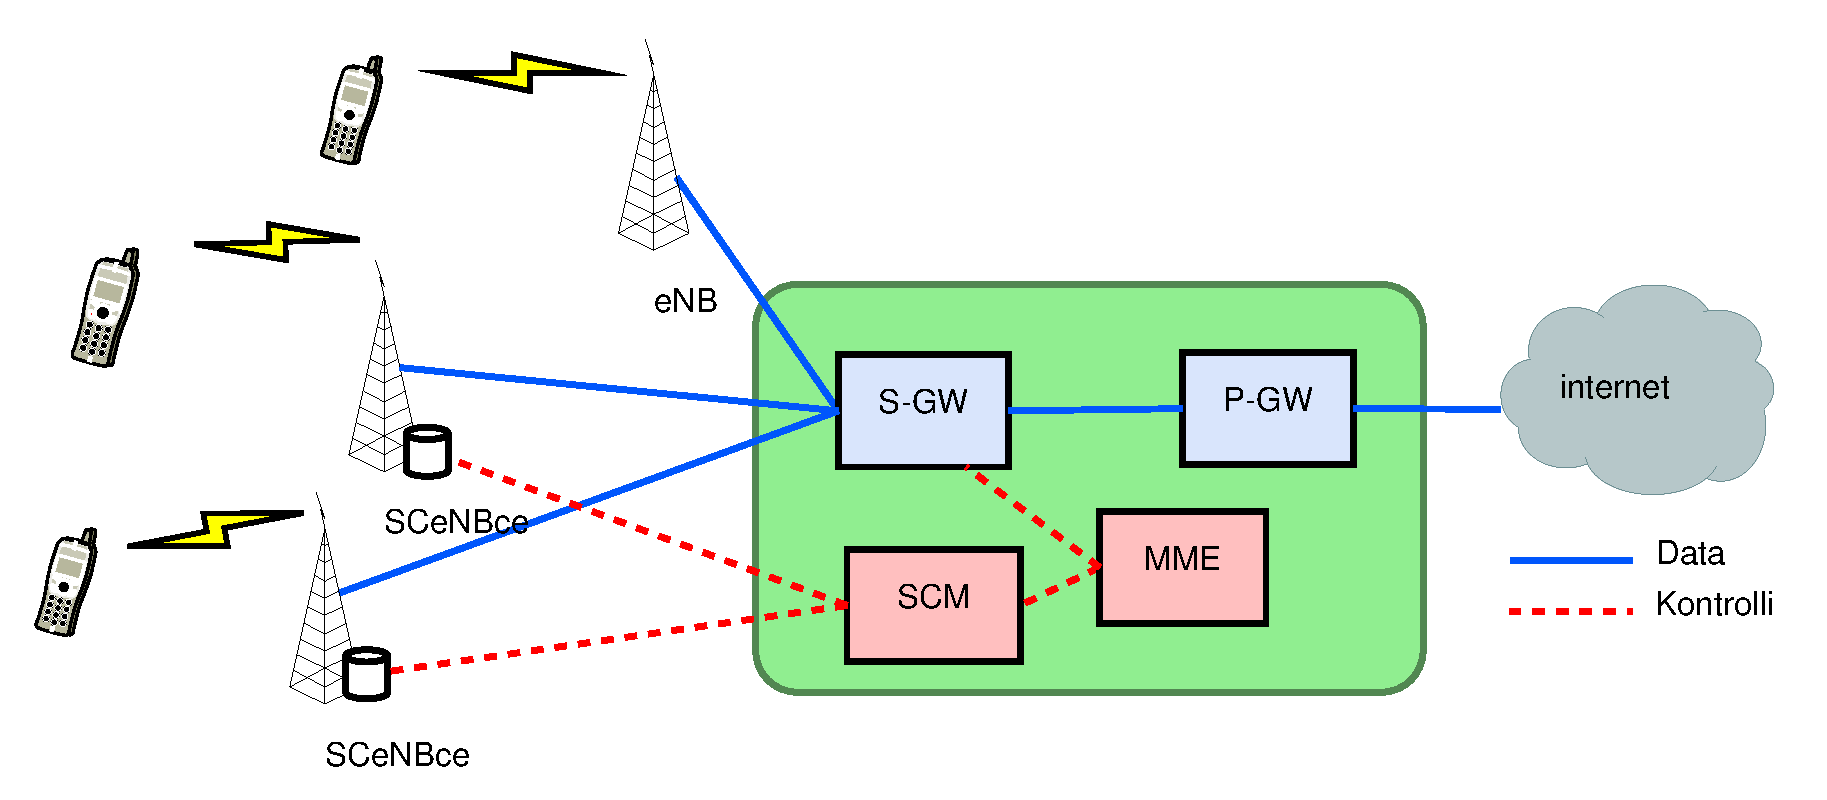
\includegraphics[width = \textwidth]{SCC.eps}
\caption{SCC arkkitehtuuri jossa SCM on integroitu osaksi EPC:tä} \label{fig:scc}
\end{figure}

\subsection{Small Cell Cloud} \label{scc}

Small Cell Cloud (SCC) on reuna-arkkitehtuuri ehdotus LTE tyyppiseen mobiiliverkkoon.
Idean premisseinä toimivat laskentaresurssien lisääminen mobiiliverkon tukiasemiin ja mobiiliverkon solujen pieneneminen.
Näillä toimilla voitaisiin vastata tietoliikenteen määrän kasvuun sekä tarjota reunalaskentaa uutena palveluna.
SCC:n ratkaisuympäristönä toimii LTE verkko, jonka kehitystä ehdotettu ratkaisu pyrkii myötäilemään.
Pienemmät solut tarkoittavat että tukiasemat sijaitsevat lähempänä asiakasta, joka puolestaan implikoi asiakaslaitteille nopeampaa tiedonsiirtoväylää radiorajapinnassa \cite{lobillo15scc}.
Seuraavaksi käsitellään SCC:n toiminnallisuus aloittaen läpikäynti toimijoista. Lopuksi käsitellään tietoliikenneratkaisuja joita SCC:n yhteydessä on ehdotettu.

SCC:ssä laskentaresurssit on sijoitettu eNodeB tukiasemiin. SCC:n tapauksessa puhutaan SCeNBce:stä (Small-cell eNodeB computing-enhanced), eli laskentaresursseilla varustetusta piensolutukiasemasta \cite{lobillo15scc}.
Reunalaskentaan käytettävät resurssit ovat integroituina osaksi tukiasemaa \cite{puente15seamless}.
Ajatuksena on että tukiaseman toiminnot suoritettaisiin samalla laitteistolla kuin reunasovellukset.
Tämänkaltainen menettely mahdollistaa tukiaseman ja reuna-alustan yhteistoiminnallisuutta.
Yhteistoiminta mahdollistaa esimerkiksi radiorajapinnasta saatavien tietojen hyödyntämisen osana etälaskennan kannattavuuden päättelyä.
Lisäksi yhteisillä jaetuilla resursseilla vältyttäisiin erillisen laitteiston lisäämiseltä \cite{puente15seamless}.

SCC:n hallinnollisista toimista vastaava entiteetti on Small Cell Manager (SCM) \cite{lobillo15scc}.
SCM olisi MME:n kaltainen itsenäinen toimija, mutta vastaisi reunalaskentaan liittyvistä hallinnollisista toimista.
Tarkoituksena on että SCM on tietoinen reunasolmujen resurssien tilasta ja on kykenevä tekemään päätöksiä reunasovelluksien siirtämisestä sijainnista toiseen. 
Lisäksi SCM:n tehtävänä on vastata muun muassa asiakaslaitteiden pyyntöihin laskentaresursseista osoittamalla käytettävissä oleva virtuaalikone \cite{dolezal2016performance}.
SCM voi myös sähkön säästämiseksi sulkea SCeNBce:n reunalaskentatoiminnallisuuden.
SCM:n sijoittelu mobiiliverkon sisällä on jätetty toteuttajan vastuulle, mutta ehdotettuja sijainteja ovat muun muassa MME:n yhteydessä ja täysin itsenäisenä toimijana \cite{lobillo15scc}.
SCM toteutusvaihtoehdot sisältävät sekä hajautettuja että keskitettyjä malleja.

SCC ympäristössä perustoiminnallisuus menisi siten että reunalaskentaa tahtova asiakaslaite välittäisi pyynnön SCeNBce:lle joka edelleen välittäisi pyynnön SCM:lle.
SCM toimii reuna-alustan roolissa ja valitsee SCeNBce:lle virtuaalikoneen, jolla reunalaskentaa voidaan suorittaa. \cite{dolezal2016performance}


Koska SCC:n ehdotetaan olevan tiukasti integroituna LTE mobiiliverkkoon, vaatii se olemassa olevien rajapintojen lisäksi uuden rajapinnan SCM vaatimien toiminnallisuuksien toteuttamiseksi. SCM tarvitsee rajapinnan MME:hen jonka kautta se voi esimerkiksi autentikoida asiakaslaitteita \cite{lobillo15scc}. 
Joskaan SCC:n käyttöönotto ei vaadi mobiiliverkon täysimittaista uudelleen rakentamista, edellyttää se toimiakseen ainakin olemassa olevien tukiasemien korvaamisen SCeNBce tyyppisillä tukiasemilla. Lisäksi käyttöönotto vaatii puuttuvien rajapintojen lisäämistä MME:n yhteyteen. 
Laskentaresurssien sijoittaminen tukiasemaan tekee resursseista hyvin paikallisesti hyödynnettäviä. Onkin siis tarkkaan pohdittava resurssien määrää tukiasemassa koska ne eivät ole kovin helposti muiden solujen hyödynnettävissä.
%täten voi oletta

 
%
%SCC:n arkkitehtuurin haasteena saattaa olla niiden ylläpidettävyys, jossa matkapuhelinverkko-operaattori on vastuussa reunasolmun ylläpidosta, koska se on tiukasti sidoksissa tukiasemaan\cite{lobillo15scc}.
%Tukiasemaan tiukasti sidotulla ratkaisulla on kuitenkin mahdollista hyödyntää laajemmin tukiaseman ominaisuuksia, kuten radioyhteyksiä toisiin tukiasemiin.
%SCeNBce tukiasemien hankkiminen vaatii operaattoreilta investointeja sekä lisää ylläpitotyön määrää. (Näiden vuoksi ehkä kantsis miettii, että miksi se on niin tiukasti kiinni siinä televerkossa. Muutenkin useampi operaattori samalla alueella tarkoittaa että jokaisella on myös omat reunapalvelut, joka taas meinaa kokonaiskuvassa että sama palvelu pitää duplikoida monelle operaattorille.)

\subsubsection{Kommunikointi reunapalveluun} \label{GTP}
Kuten kappaleessa \ref{kommunikaatio} käsiteltiin, tavallisesti asiakaslaitteen tietoliikenne kulkee mobiiliverkon läpi koskemattomana GTP tunnelin sisällä. 
SCC:n asiakaslaitteen ja reunalaskennan välisen tietoliikenteen reititys on esitelty julkaisussa \cite{puente15seamless}, johon tämä kappale pohjautuu.
SCC:n tapauksessa asiakaslaitteen liikenne haluttaisiin ohjata kohteesta riippuen joko tukiasemassa sijaitsevalle reunasolmulle tai normaalia reittiä pitkin ulkoverkkoon.
SCC:ssä on päädytty lisäämään SCeNBce tukiasemaan tietoliikennettä monitoroiva toiminnallisuus.

Kommunikaatio asiakaslaitteen ja tukiaseman välillä suoritetaan DRB väylällä (Data Radio Bearer).
Perinteisesti tukiasema identifioi asiakaslaitteet radiorajapinnassa DRB ID:n (Data Radio Bearer ID) avulla.
Tämän jälkeen asiakaslaitteen tietoliikenne on tukiasema kapseloi asiakkaan tietoliikenteen GTP tunneliin, jonka tunnisteena toimii TEID (Tunnel Endopoint ID).
Asiakaslaitteen tietoliikenteen välitys tukiaseman sisällä vaatii siis DRB ID:n ja TEID:n sisältävän muunnostaulun käyttämistä.
Tätä samaa periaatetta voi hyödyntää reunasolmulle suuntautuvan tietoliikenteen identifiointiin.

Tukiasemaan lisättävän monitoritoiminnallisuus tarkkailee asiakaslaitteen lähettämien pakettien kohde IP-osoitetta, ja mikäli kyseessä on reunapalvelun IP-osoite, monitori ohjaa paketin reunapalvelulle.
Samalla paketista voidaan poimia asiakaslaitteen IP-osoite, joka kirjataan muunnostauluun asiakasta vastaavan TEID:n ja DRB ID:n kanssa.
Toiseen suuntaan tietoliikenne toimii siten että reunapalvelun asiakaslaitteelle lähettämästä tietoliikenteestä poimitaan kohde IP. Kohde IP:tä vastaava DRB ID poimitaan muunnostaulusta reunapalvelun paketit kapseloidaan DRB väylälle sopiviksi.
Tällaisen toiminnallisuuden toteuttamisen seurauksena kommunikaatio on asiakaslaitteen ja reunapalvelun näkökulmasta kuin mikä tahansa muukin IP-pohjainen kommunikaatio.

Asiakaslaiteen ja reunasolmun välisen kommunikaation säilymiseen, tilanteessa, jossa asiakaslaite siirtyy toiselle tukiasemalle, ei oteta kantaa. 
Tällaisen toiminnallisuuden tarve kuitenkin on, sillä SCM esittelyn yhteydessä mainittiin reunasovelluksien, eli virtuaalikoneiden, siirtelyn mahdollisuus.
%SCC pohjaisessa järjestelmässä tavallinen verkkoon menevä tietoliikenne ja reunapalvelulle menevä tietoliikenne on ehdotettu eroteltavaksi toisistaan \cite{puente15seamless}.
%Eristyksen seurauksena LTE-A arkkitehtuuriin ei tarvitse koskea muutoin kuin lisäyksien osalta. 
%Liikenne SCeNBce:llä tarjottuihin reunapalveluihin on tehtävä tarkoitusta varten olevan rajapinnan kautta.
%Asiakaslaitteelta tuleva liikenne reititetään SCeNBce:llä. 
%Pakettien reitittämiseksi SCeNBce joutuu päättelemään, onko paketin määränpää reunapalvelu vai tavallinen tietoliikenne.
%
% Koska LTE-tukiasemat eivät toimi IP tasolla, ei reunapalvelulta tuleva pakettiliikenteen sisältämä asiakaslaitteen IP-osoite riitä identifioimaan kohdelaitetta. 
%Yleisesti LTE verkossa, internetistä asiakaslaitteelle suuntautuvan liikenteen osalta pakettien ohjaamiseksi, käytetään GTP-tunnelia. GTP-tunnelilla tietoliikenne saadaan ohjattua oikealle tukiasemalle.
%Tukiaseman ja asiakaslaitteen välisen kommunkaatioväylän selvittämiseksi joudutaan tekemään TEID (Tunnel endpoint IDentifier) ja DRB-ID (Data Radio Bearer ID) muunnos.
%
%Vastaava ongelma on myös reunapalvelulta asiakaslaitteelle suuntautuvassa tietoliikenteessä.
%SCC:n yhteydessä ehdotetussa ratkaisussa reunapalvelulta tulevan liikenteen yhdistäminen asiakaslaitteen IP-osoitteeseen voidaan tehdä käyttäen TEID perustuvaa ohjaustaulua.
%TEID on asiakaskohtaisen GTP-tunnelin indetifioiva tunniste.
%TEID:stä ja asiakaslaitekohtaisesta IP-osoitteesta voidaan muodostaa SCeNBce:lle reititystaulu. 
%Reititystaulun avulla voidaan ohjata IP-osoitte muuntaa DRB liikkenneväyläksi ja ohjata tietoliikenne asiakaslaitteeseen.


 
\subsection{SMORE ja MobiScud}
SMORE (Software defined network Mobile Offloading aRchitecturE) on toinen televerkkoihin suunniteltu MEC ratkaisu. \cite{cho2014smore}
SMORE:n keskeisin sisältö on ottaa SDN (Software Defined Networking) käyttöön reunapalveluiden saavuttamiseksi. SDN käyttöönotolla tavoitellaan sitä, että televerkon toimintaan ei tarvitsisi tehdä muutoksia. Minkään olemassa olevan komponentin toiminta ei siis muutu. 
SMORE:n toiminta on jaettu kahteen osaa, joita varten SDN on käytössä. 
Ensimmäisenä on mobiiliverkon kontrollitasolla (control-plane) tapahtuva viestien monitorointi. 
Toisena toimintona on monitoroitujen tietojen pohjalta tehtävät SDN hallintatoimenpiteet. Näiden avulla voidaan ohjata haluttu osa tietoliikenteestä haluttuihin reunalaskentayksikköihin.
Kontrollitasolla viestejä monitorointia suorittaa SMORE monitori (SMORE monitor) ja tietoliikenteen ohjauspäätöksistä vastaava komponentti on SMORE kontrolleri (SMORE controller).

Tietojen välitys SMORE kontrollerin ja SMORE monitorin välillä on toteutettu yhteisen tietokannan kautta. SMORE monitor tallentaa poimitut tiedot tietokantaan ja antaa tiettyjen tapahtumien yhteydessä SMORE kontrollerille herätteen tehdä asianmukaiset muutokset SMORE:n SDN reitityksiin. Herätteitä laukaisevat tapahtumat ovat asikkaan liittyminen verkkoon ja asikkaan liikkuminen verkossa.

SMORE monitori tarkkailee asiakaslaitteen ja LTE/EPC:n välistä liikennettä.
Asiakaslaitteen liittyessä mobiiliverkkoon, asiakaslaite ja LTE/EPC:n sisäiset komponenti muodostavat tunneleita ja asiakaslaitteeseen liitetään erilaisia tunneleita koskevia osoite ja metatietoja.
SMORE monitorin tehtävänä on poimia asiakaslaitteen liittyessä ja yhteydenmuodostuksen aikana asiakaslaitteisiin liittyviä tietoja.
Asiakaslaitteen lähettäessä liittymispyynnön (attach request) SMORE monitori poimii pyynnöstä asiakaslaitteen IMSI (international Mobile Subscriber Identity) ja TAI:n (Tracking Area Identifier). 
Tämän jälkeen SMORE monitori poimii MME:n asiakaslaitteelle lähettämästä liittymispyynnön hyväksymis -viestistä (attach accept) monitori poimii asiakaslaitteelle annetun IP-osoitteen, SGW:n IP-osoitteen, SGW:n TEID:n ja asiakaslaitteen GUTI:n (Globally Unique Temporary Id).
Tämän jälkeen eNodeB neuvottelee asiakaslaitteen kanssa radioyhteydestä ja tämän lopputulos välitetään MME:lle. SMORE monitor poimii eNodeB:n ja MME:n välisestä kommunikaatiosta eNodeB:n IP-osoitteen ja eNodeB:n TEID:n.
Kun edellä mainitut tiedot on tallennettu SMORE:n tietokantaan, SMORE monitor lähettää SMORE kontrollerille herätteen päivittää SDN reitityksiä. 

Toinen tapahtuma josta SMORE kontrolleri on kiinnostunut on handover, eli mikäli asiakaslaite siirtyy mobiiliverkossa eNodeB:den välillä. SMORE kontrollerin on tässä tapauksessa kiinnostunut mobiiliverkossa tapahtuvista muutoksista. 
Handover alkaa kun tällä hetkellä käytössä oleva eNodeB päättää, että on aika siirtää asiakaslaitteen yhteys toiselle eNodeB:lle (kohde).
Alkuperäinen eNodeB välittää pyynnön kohteena olevalle eNodeB:lle joka oletettavasti hyväksyy sen. Tämän jälkeen, kohteena oleva eNodeB pyytää MME:ltä reitityksen muutosta. Tässä välissä oleva SMORE monitor poimii reitityksen muutosta koskevan tiedon ja välittää ne SMORE kontrollerille.
Tämän tiedon pohjalta SMORE kontroller voi tehdä SDN muutokset siten että vanhat reititykset voidaan poistaa ja korvata uusilla.


\subsubsection{MobiScud}
MobiScud \cite{wang2015mobiscud} on SMORE:n ideoita ammentava versio reunalaskentapalveluiden tuottamisesta mobiiliverkoissa.
MobiScud:in perustoiminnallisuus on hyvin samankaltainen kuin SMORE:ssa. MobiScud painottaa enemmän käyttäjän tarvetta liikkua verkossa. Lisäksi MobiScud käyttää hyödykseen oletusta mobiiliverkkojen hajautettua rakennetta. 

Kuten SMORE, MobiScud käyttää hyödykseen SDN:n tarjoamia ominaisuuksia ja siten olettaa sen käyttöönottoa palveluntarjoajan infrastruktuurissa. Lisäksi MobiScudin toiminnallisuudet on ajateltu toteutettavan Network Function Virtualisantionin (NFV) avulla. 
MobiScud Controller (MC) koostuu kahdesta loogisesta kokonaisuudesta: monitorista ja kontrollerista. Näiden toimintaperiaate on käytännössä identtinen SMORE:n vastaavan nimisiin toimijoihin. MC:n sijaintia ei kuitenkaan ole keskitetty kuten SMORE:ssa vaan sen oletetaan sijaitsevan hajautettna RAN ja EPC välissä.
Käyttäjän ja reuna-infrastruktuurin välinen yhteys toteutetaan hyvin samalla tavalla kuin SMORE:ssa. 

MobiScudin reunapalvelut on ajateltu toteutettavan hyvin cloudletmäisesti. Mahdollisimman lähellä reunaa sijaitsevassa "pilvessä" on palvelinresursseja, joita käyttäjät hyödyntävät yksityisien virtuaalikoneinstanssien muodossa (Private Virtual Machinem, PVM). 

MobiScudin tavoitteena on tarjota asiakkaalle mahdollisimman nopea yhteys asiakkaan ja PVM:n välille. MobiScud hyödyntää televerkon omia kontrollitason viestejä asiakkaan liikkumisen seuraamiseen. Kun handoverista tulee viesti MC:n monitoroivalle entiteetille, alkaa MC organisoimaan reunalaskentaan liittyviä muutoksia. 

Asiakkaan siirtyessä tukiasemalta toiselle PVM:n siirto aloitetaan livemigraationa kohteena olevalle "pilvelle". Livemigraation ollessa käynnissä kohteena olevan pilven MC huolehtii että asiakaslaitteella on edelleen yhteys alkuperäiseen sijaintiinsa. Tämä hoidentaan SDN reititysmuutoksilla. Kun PVM:n livemigraatio on saatu suoritettua alkuperäisen sijainnin MC ilmoittaa tästä kohdesijainnin MC:lle, joka puolestaa päivittää SDN reititykset ohjaamaan siirretylle PVM:lle.

MobiScudin testeissä livemigraation ja SDN reitityksien avulla RTT (round trip time) saatiin pidettyä pienenä. Kuitenkin yhteyksissä aiheutui noin kahden sekunnin mittaisia katkoksia sillä hetkellä kun livemigraation viimeiset muutokset lähetetään. Yhteyskatkoksen pituuteen vaikuttavat monet asiat ja artikkelissa huomautetaankin että nykyinen toteutus oli optimoimaton ja vaatii jatkotutkimuksia.



\subsection{CONCERT}
Nykyinen LTE televerkko koostuu joukosta laitteita, joilla on hyvin spesifit tehtävät. CONCERT \cite{liu2014concert} pyrkii seuraavan sukupolven televerkkoihin keskittyvässä ratkaisussaan vähentämään tehtäväspesifien laitteiden tarvetta. 
CONCERT arkkitehtuuri koskee siis pääasiassa seuraavan sukupolven televerkkoja, vaikkakin sen ratkaisut mahdollistavat tuen myös vanhemmille teknologioille. CONCERT esittää uudenlaista toiminnallisuuksien toteuttamismallia, joka korvaisi valmistajakohtaisia telelaitteita (kuten tukiasemat) virtualisoiduilla ja ohjelmistopohjaisilla ratkaisuilla. NFV ja SDN käyttöönotto toimii siis tämänkin ehdotuksen selkärankana.
Verkon toimintojen virtualisointi mahdollistaa laitteiston siirtämisen kauemmaksi reunasta, joka osaltaan vähentää hajautettavan laitteiston määrää. CONCERTin ideana on, että hajautetuksi jäisi telelaitteistosta ainoastaan välttämättömin osa, eli radiorajapinnan mahdollistava RIE (Radio Interfacing Equipment) ja hierarkisesti jaetut reunalaskentayksiköt. Televerkon muita toiminnallisuuksia voitaisiin keskittää ja tarjota virtuaalisina ohjelmistoteutuksina. 

Conductor on CONCERT arkkitehtuurissa hallinnollisessa keskiössä ja se vastaa päällysverkon hallinnasta.
CONCERT arkkitehtuurissa control ja data planet on erotettu toisistaan ja Conductorin tehtävänä esittää data planella esiintyvät fyysiset resurssit virtuaalisina resursseina.
Reunalaskentayksiköiden resurssien jakaminen sekä niiden välisten SDN kytkimien kautta muodostettujen yhteyksien hoitamisesta vastaa conductor.
Conductorin toiminta on toistaiseksi kuvattu vain korkealla tasolla, joten sen toteutustekniset ratkaisut ovat avoimia.

Vaikka laitteiston virtualisointi ja palveluiden keskittäminen kustannuksien säästämiseksi kuulostaakin houkuttelevalta, on kesittämisessä myös omat ongelmansa.
Etenkin liiallinen keskittäminen siirtää verkon toiminnallisuuksia kauemmaksi reunasta, joka osaltaa johtaa korkeampiin latensseihin ja heikentää palvelun laatua. Vaikka conductor onkin esitetty yksittäisenä loogisena entiteettinä, sen toiminnallisuuksia on mahdollista porrastaa ja hajauttaa paremman skaalautuvuuden ja pienempien latenssien tavoittamiseksi.

CONCERTin ratkaisu reunapalveluiden tuottamiseksi on hierarkinen kolmeen tasoon jaettu arkkitehtuuri.
\textit{Paikalliset} reunalaskentaresurssit sijaitsevat kaikkein lähimpänä verkon reunaa, esimerkiksi RIE:n kanssa samassa sijainnissa sijaitseva palvelin. Paikallisen reunalaskentayksikön laskentaresurssit ovat rajalliset ja sen tehtävänä onkin suorittaa ainoastaan kaikkein tiukimman aikavaatimuksen laskentaa.
\textit{Alueelliset} reunalaskentaresurssit kattavat jonkin pienen alueen reunalaskenta tarpeita ja korkeimman tason \textit{keskus} reunalaskentaresurssit kattavat jonkin suuremman alueen resurssi intensiivistä reunalaskentaa.
CONCERT:ssa reunalaskentaresurssien jakamisesta vastaa conductorin sisäinen komponentti LCM (Location-aware computing management).


 Reunalaskennan osalta CONCERTissa resurssit on jaettu hierarkisesti kolmeen tasoon, siten että lähimpänä käyttäjää on \textit{paikalliset} palvelimet, jotka on tarkoitettu kaikkein tiukimman aikavaatimuksen sovelluksille. Seuraavat kaksi tasoa, \textit{alueellinen} ja \textit{keskus (central)}, kasvattavat palvelinresurssien määrää, mutta ovat kauempana reunasta. Reunalaskentayksiköt voivat olla yhteydessä toisiinsa, jolloin ne mahdollistavat nopeat M2M (Machine-to-Mahcine) yhteydet. Tämä mahdollistaisi muunmuassa autojen välisen kommunikaation reunaverkon välityksellä. 

Toistaiseksi CONCERT on korkean tason suunnitelma ja se käyttää hyväkseen vielä olemassa olemattomia teknologisia ratkaisuja kuten tukiasemien virtualisointia. Arkkitehtuuri mahdollistaa erilaisien ratkaisujen toteuttamisen, eikä aseta tiukkoja rajoitteita resurssien tai hallinnon sijoittelun suhteen.



\subsection{ETSI MEC}
ETSI (European Telecommunications Standards Institute) on eurooppalainen telealan standardointijärjestö.
ETSI on aloittanut reunalaskennan arkkitehtuurin, sekä sen touteuttamiseksi vaadittavien toimintojen standardoimisen.

ETSIn MEC spesifikaatio määrittelee reunapalvelun tuottamiseksi vaadittavat ominaisuudet, jotka reunainfrastruktuurin tulee toteuttaa.
Spesifikaatio listaa myös mahdollisia, mutta ei vaadittuja toimintoja. 
Listaamalla vaaditut toiminnot stanrardi pyrkii yhtenäistämään reunalaskennan konsepteja.  

\subsubsection{Vaatimukset}
Vaatimukset on jaettu kategorioihin sen mukaan mihin toiminnallisuuteen vaatimus liittyy.
Vaatimuksien kategoriat ovat yleiset vaatimukset (generic requirements), palvelu vaatimukset (service requirements), hallinta vaatimukset (operation and management requirements) ja viimeisenä kategoriana on kokoelma vaatimuksista, joiden teemoina ovat turvallisuus, sääntely ja veloitus (Security, regulation, charging requirements)\cite{etsitechreq}. 

Yleiset vaatimukset ovat luonteelta korkean tason kuvauksia reuna-infrastruktuurin toiminnallisuuksista. Yleiset vaatimukset kategorisoitu seuraaviin luokkiin: viitemallista, reunapalvelun sovelluksien elinkaaresta (application lifecycle),
reunapalvelun sovellusympäristöstä (application enviroment) sekä liikkuvuuden tuesta (support of mobility).
Viitemallin tulee vaatimuksien mukaan hyödyntää mukaan NFV ratkaisuja hallinnollisten toimien toteuttamiseen, mikäli mahdollista. 
ETSI:n vaatimuksen mukaan reunapalvelun tulee voida sijaita käytännössä missä tahansa kohdassa radiomaston runkoverkon reunan välillä. Sijainnin vapaus myös tarkoittaa että reuna-alusta(?) ei voi olla riippuvainen alla olevasta infrastruktuurista. 
Reunapalvelun sovelluksien elinkaareen liittyvät vaatimukset koskevat pääasiassa reunapalvelun toimijoiden oikeuksia päättää reunan sovelluksien käynnistämisestä ja sulkemista.
Reunapalveluiden sovellusympäristöä koskevissa vaatimuksissa esitetään, että sovelluksien autenttisuus ja eheys pitää pystyä varmentamaan. Sovellusympäristön täytyy myös mahdollistaa reunasovelluksen käyttöönotto toisella reuna-isännällä, ilman erikoisempaa mukautusta (without specific adaptation) \cite{etsitechreq}.
Mobiiliverkkojen ollessa kyseessä, asiakaslaitteiden liikkuminen tukiasemalta toiselle, on keskeinen käyttötapaus. Tämä heijastuu myös vaatimukseen liikkuvuuden tukemisesta reunapalveluissa.
Vaatimuksena on että asiakaslaitteen ja reunapalvelun välisen yhteyden tulee säilyä, vaikka asiakaslaite siirtyisi solusta toiseen tai asiakaslaite siirtyisi sellaiseen soluun joka on toisen reuna-isännän vastuualuetta.

Palveluvaatimukset on joukko vaatimuksia, jotka keskittyvät takaamaan reuna-infrastruktuurin perimmäiset palveluperiaatteet.
Lista palveluvaatimuksista on pitkä, joten tähän tutkielmaan on poimittu ainoastaan osa vaatimuksista. Täydellinen lista löytyy \cite{etsitechreq} julkaisusta.
Palveluvaatimukset kuvaavat toiminnallisuuksia, joiden avulla reunapalveluita voidaan tuottaa. Tällaisesta esimerkkinä tietoliikenteen reitittämiseen liittyvät vaatimukset, joiden keskeinen tehtävä on kuvata mahdolliset tietoliikennereitit reunapalveluun ja ulos reunapalvelusta. Yksi ehkä keskisimmistä palveluvaatimuksista on reuna-alusta mahdollisuus suodattaa ja muokata verkkoliikennettä. 
Lisäksi kuvataan että reunapalveluiden toimintaa ei haluta rajoittaa pelkästään asiakas-palvelu tyyppisen toimintamalliin. Reunapalveluiden tuottamiselle onkin annettu mikropalvelu -tyyppinen (microservice) kuvaus, jossa palveluntuottajat voivat toimia myös toisten reunapalveluiden kuluttajana (consumer).

\subsubsection{Viitekehys ja referenssiarkkitehtuuri}

ETSIn esittämän viitekehys esittää reunalaskentaan liittyvät korkean tason entiteetit. Nämä entiteetit on jaettu kolmeen tasoon: järjestelmä, isäntä ja verkko(system, host ja network). 
Verkkokerros sisältää verkkoyhteyksistä vastaavat entiteetit. MEC:n tapauksessa verkkokerros koostuu ainakin kolmesta osasta: sisäverkko, ulkoverkko ja televerkko.
Isäntäkerros koostuu reunapalveluiden virtualisointiin ja reunapalvelun hallinointiin keskittyvistä entiteeteistä.
Järjestelmäkerros koostuu korkeamman tason hallinnosta vastaavista elementeistä.

Referenssiarkkitehtuurissa on esitetty funktionaaliset entiteetit. Funktionaalisten entiteettien toiminta on kuvattu 
Referenssiarkkitehtuurissa reuna-isännällä (edge-host) tarkoitetaan entiteettiä, joka tarjoaa virtualisointi-infrastruktuurin, sekä reunalaskennan toteuttamiseen vaadittavat resurssit (laskenta, tallennus ja verkko).
Reuna-alustalla (Mobile edge platform) tarkoiteen sitä entiteettiä joka mahdollistaa reunapalveluiden käyttämisen. Reuna-alusta siis mahdollistaa reunapalveluiden saavuttamisen, eli käytännössä tarjoaa rajapinnan asiakaslaitteen suuntaan. Tähän kuuluu siis palvelurekisterin ylläpitäminen, reitityssääntöjen ylläpitäminen, sekä liikenteen välittäminen reunapalveluille. Reuna-alusta voi myös itse tarjota  palveluita.
Esimerkkinä tällaisesta voisi olla tunnistautumispalvelu. 
Reuna-applikaatioilla tarkoitetaan reuna-alustalla suoritettavia virtuaalikoneita, jotka suorittavat reunapalveluiden tuottamiseksi tarkoitettuja ohjelmistoja.


\subsection{Vertailu}

% Taulukko toiminnoista

\begin{table}
	\caption{Reunalaskenta-arkkitehtuurien ominaisuudet}
	\label{table:features}
	
\end{table}
 
\bibliographystyle{apalike}

\bibliography{lahteet}

\lastpage

% --- Appendices ---

% uncomment the following

% \newpage
% \appendix
% 
% \section{Esimerkkiliite}

\end{document}
